\documentclass[ a4paper,
                oneside,
                toc=bibliography,
                toc=listof
                ]{scrbook}


% set the language here. Last language is the main language. Use `ngerman` (= new german) for German texts.
\usepackage[ngerman, english]{babel}
% \usepackage[english,ngerman]{babel} % If your text mainly is in German.



% general math support
% consider using bracket environments for inline math, i.e. \(x_2^2 + \sqrt{\gamma}\) instead of $$.
% for numbered equations in their own line, use e.g. the array environment. 
\usepackage{amsmath, amssymb}

% bold math package. Set matrices and vectors with \bm{v}
\usepackage{bm}

% beautiful table environments (see https://ctan.org/pkg/booktabs)
\usepackage{booktabs}

% multi page table. Your list of symbols may need this
\usepackage{longtable}

% consistent acronym definitions and usage. You may want to use the glossaries package instead, which is more powerful, but more complex to handle.
\usepackage[printonlyused, smaller]{acronym}

% for multiple plots in one figue, e.g. Fig 1.a and Fig 1.b
% https://en.wikibooks.org/wiki/LaTeX/Floats,_Figures_and_Captions#Subfloats
\usepackage{subcaption}

% provides \FloatBarrier to prevent floats past some point.
\usepackage{placeins}

% For vector graphics and MATLAB figures, you may try TikZ:
% There is also tikz-uml for UML diagrams
\usepackage{tikz}
\usepackage{pgfplots}

\pgfplotsset{
    compat = newest,
	grid=major,
	every axis plot/.append style={very thick},
}

% block diagrams with tikz
\usetikzlibrary{calc,fit, positioning,arrows.meta}
\tikzset{>={Latex[width=2mm,length=2mm]}} % more visible default arrow heads
\tikzstyle{block} = [draw=black, fill=white, rectangle, align=center, minimum height=2em, minimum width=3em]
\tikzstyle{sum} = [draw, circle, node distance=1cm]

% global matlab2tikz options for exporting MATLAB plots
% https://github.com/matlab2tikz/matlab2tikz
\newlength\figureheight 
\newlength\figurewidth 
\setlength\figureheight{3cm} 
\setlength\figurewidth{0.7\textwidth}


% If you want to use colors, we already defined some for you (university corporate design)
\RequirePackage{xcolor}

\definecolor{UStuttDarkBlue}{RGB}{0,81,158}
\definecolor{UStuttLightBlue}{RGB}{0,190,255}
\definecolor{UStuttDarkGreen}{RGB}{59,140,122}
\definecolor{UStuttLightGreen}{RGB}{125,155,101}
\definecolor{UStuttDarkOrange}{RGB}{228,175,52}
\definecolor{UStuttLightOrange}{RGB}{236,218,145}


% for code listings, you can e.g. use the "listings" package (http://texdoc.net/texmf-dist/doc/latex/listings/listings.pdf):
\usepackage{listings} 
\usepackage{scrhack} % if you load listings together with scrbook etc., then load this fixing package as well

\lstset{
  captionpos=b,
  commentstyle=\color{UStuttDarkGreen},
  frame=single,	                   % adds a frame around the code
  keepspaces=true,
  %keywordstyle=\color{UStuttDarkBlue},
  showspaces=false,
  showstringspaces=false,          % underline spaces within strings only
  showtabs=false,
  stringstyle=\color{UStuttDarkBlue},
  tabsize=2
}


% This class does the ISW styling for you (together with scrbook).
%
% It handles the following:
% - Proper input and font encoding (Just type, don't care about the LaTeX compiler you use or how to type German umlauts)
% - Fonts with ligatures and kerning (Tex Gyre fonts are used, part of every LaTeX installation, text is nice to read)
% - Bibliography styling for biblatex (declare your bibliography file and you are ready to go)
% - Provide command for title page (\makeISWtitle) and declaration of originality ( \declarationOfOriginality)
% - Loads packages "biblatex" and "graphics"
\usepackage[
    type=MA, % BA, MA, FA, SA (old), bachelorproject
]{iswthesis}

% hyperref provides hyperlinks within the document, but also auto-naming.
% E.g. when referencing, instead of typing "Figure~\ref{fig:XY}" try "\autoref{fig:XY}".
% You may want to use `clevceref` instead of using \autoref in the hyperref package, which has slightly more possibilities.
\PassOptionsToPackage{pdfpagelabels}{hyperref}
\usepackage{hyperref}  % backref linktocpage pagebackref
\pdfcompresslevel=9
\pdfadjustspacing=1

\hypersetup{%
    %draft, % = no hyperlinking at all
    %colorlinks=true,
    colorlinks=false, 
    linktocpage=false, pdfborder={0 0 0},%
    breaklinks=true, pdfpagemode=UseNone, pageanchor=true, pdfpagemode=UseOutlines,%
    plainpages=false, bookmarksnumbered, bookmarksopen=true, bookmarksopenlevel=1,%
    hypertexnames=true, pdfhighlight=/O,%nesting=true,%frenchlinks,%
    %urlcolor=Black, linkcolor=Black, citecolor=Black, %pagecolor=Black,%
} 


% Your own commands (https://en.wikibooks.org/wiki/LaTeX/Macros):
% Consider defining your own commands for often used terms, e.g.

% Real numbers symbol
\newcommand{\R}{\mathbb{R}}

% Transpose of vector or matrix (upright)
\newcommand{\T}{\mathrm{T}}

\newcommand{\mustbe}{\ensuremath{\stackrel{!}{=}}}

% short matrix environment. Instead of typing \begin{bmatrix} 1 & 2 \\ 3 & 4 \end{bmatrix} you can now use as well \bmat{1 & 2 \\ 3 & 4}
\newcommand{\bmat}[1]{ \ensuremath{\begin{bmatrix} #1 \end{bmatrix}} }

% partial derivative: \partfrac{^2}{x^2} yields ∂²/∂x²
\newcommand{\partfrac}[2]{ \ensuremath{\frac{\partial #1}{\partial #2}} }

% upright "d" for differentiation
\newcommand{\ddiff}{\ensuremath{\mathrm{d}}}

% d/dt
\newcommand{\ddt}{\ensuremath{\frac{\ddiff}{\ddiff t}}}


%pdflatex -> Biber -> pdflatex*2
% Path to .bib file for BibLatex
\addbibresource{bibliography.bib}
% \addbibresource{someOtherBibFile}

\author{Ouyang Shengzhe}
\placeOfBirth{Stuttgart}
\address{Seidenstraße 36, 70174 Stuttgart}
\major{Engineering Cybernetics}
\title{Deep learning based graph extraction from branched deformable linear objects}
\titleTranslated{Deep Learning basierte Graph Extraktion von verzweigten biegeschlaffen Objekten}
\matrnr{1234567}
\date{\today}
\supervisor{My supervisor, M.Sc.}
\professor{Prof. Dr.-Ing. Oliver Riedel}

\begin{document} 
    \frontmatter
    \makeISWtitle

	\cleardoublepage
	\setcounter{page}{1} % start at page (i) after title page
    \declarationOfOriginality

    % Kurzfassung/Abstract
    \cleardoublepage

% Start with German abstracrt
\begin{otherlanguage}{ngerman}
\chapter*{Kurzfassung}
\addcontentsline{toc}{chapter}{Kurzfasung}

Deutsche Kurzfassung hier.

\vfill
\noindent\textbf{Stichwörter:} Hamster, Training, Anleitung
\vfill
\end{otherlanguage}
% Then continue with the english one.
\begin{otherlanguage}{english}
\chapter*{Abstract}
\addcontentsline{toc}{chapter}{Abstract}

Add the english abstract here.

\vfill
\noindent\textbf{Keywords:} hamster, training, guide
\vfill
\end{otherlanguage}
    
    \cleardoublepage
    \currentpdfbookmark{\contentsname}{Inhalt}
    \tableofcontents
       

    \mainmatter
    % ********************************************************************
    % Write your own contents here:
    % ********************************************************************
    
    % TODO: remove this \nocite{*} command. This is only to demonstrate the bibliography
    %\nocite{*}


    \chapter{Introduction}

The aim of student theses is to show that students are able to work on tasks from their own field independently and according to scientific methods and that they can present their results appropriately. 
These objectives, defined in the examination regulations, raise a number of questions:

\begin{itemize}
\item What does "working according to scientific methods" actually mean?
\item What belongs to the proper presentation of results?
\item Which standards and guidelines apply at the \ac{ISW}?
\item What is to be considered in general when writing student theses at the \ac{ISW}?
\end{itemize}

Read the guidelines for the preparation of student theses at ISW! The chapters used in this template are for inspiration only. Each thesis is different and the chapter headings and their order should be adapted accordingly.

    \chapter{Literature}
    In this chapter, some basic knowledge of deep learning neural network for vision tasks, i.e. keypoints detection, will be introduced at the beginning. 
    More specifically, Some works about Wire harness detection using AI method will be presented. Additionally, some state of the art methods and architectures, 
    which might improve the precision of keypoints detection of wire harnessed will also be presented. After that, some approaches for generating datasets 
    artificially and expanding datasets are introduced at the end.
\section{Deep neural network for vision tasks}
    Recently, using deep neural network for vision tasks becomes a popular choice for researchers, for example, Image Classification\cite{8016501}, 
    Object detection\cite{10028728}, Human pose estimation\cite{Sun_2019_CVPR}, Semantic Segmentation\cite{HAO2020302}. Compare with the some 
    tradition computer vision technologies, the approach provide more satisfactory results\cite{voulodimos2018deep}. 
    In this section, some of the most important deep learning network structures for vision tasks will be introduced. Object and keypoints
    detection will be the highlights due to their close connection with the tasks of the thesis.\\
\subsection{Object detection and segmentation}
    The goals of object detection are: what(classification) and where(locolization) is the object is. \autoref{fig:object detection} is an example of object
    detection. In this image, the branches of wire harness is bounded by a green box as groundtruth. They are classified as branches and the locations could 
    also be detected. It serves as the basic of some deep learning based computer vision task such as instance segmentation and object tracking\cite{10028728}. 
    \begin{figure}
        \centering
        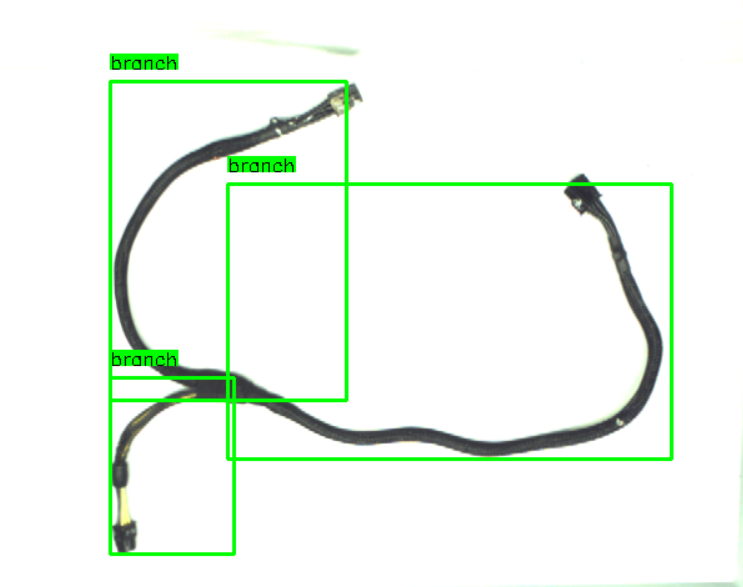
\includegraphics[width=0.6\linewidth]{example_images/object detection}
        \caption{Ground truth of Object detection}
        \label{fig:object detection}
    \end{figure}
    In \cite{Girshick_2014_CVPR}, the authors present a method called R-CNN(Region-based Convolutional Network), which improves the accuracy of object detection. 
    The approach consists of three modules:
    \begin{itemize}
        \item [(1)] \textbf{Region proposals: }In this module, category-independent region proposals will be generated.
        \item [(2)] \textbf{Feature extractions: }The features will be extracted using CNN \cite{NIPS2012_c399862d}.
        \item [(3)] \textbf{Classification: }At last the classification task is done by a set of classspecific linear SVMs. 
    \end{itemize}
    After one years, Ross Girshick proposed an optimized method named Fast R-CNN in 2015\cite{Girshick_2015_ICCV}. Compared with all objects on image are passed 
    through the neural network in R-CNN,  in Fast R-CNN the whole images will be passed forward together to extract the features, which improves the efficiency 
    significantly. Faster R-CNN combined Fast R-CNN with Region Proposal Networks(RPN), which outputs a set of rectangular object proposals, each with an objectness
    score\cite{NIPS2015_14bfa6bb}. It is trained end-to-end to generate high-quality region proposals, which are passed to Fast R-CNN for object detection tasks.
    This method simplified the process further and the model is easier to be trained.\\
    The above introduced models are from R-CNN family. Joseph Redmon proposed a new model named YOLO, whose pipeline has just one simple network. It could also be 
    trained end-to-end extremely fast\cite{Redmon_2016_CVPR}. The detection task will be framed as a regression problem to spatially separated bounding boxes and
    associated class probabilities. Due to the rapidity, it is widely used in the task of real-time object detection. After an eight-year development, the Tsinghua 
    University team presented the tenth generation of the YOLO model in 2024\cite{wang2024yolov10}. Today, the YOLO model integrates state-of-the-art deep learning 
    techniques, such as an enhanced version of CSPNet\cite{Wang2019CSPNetAN} as the backbone network, PAN (Path Aggregation Network) for effective multi-scale feature
    fusion\cite{Liu_2018_CVPR}. This enables fast and accurate real-time object detection.
    Kaiming He from Facebook AI Research extended Faster R-CNN\cite{NIPS2015_14bfa6bb} with a new branch for predicting the mask of objects\cite{He_2017_ICCV}. Therefore, it is widely 
    used in the field of instance segmentation. This method has also two stages. The predictions of mask and classification are in parallel. This is different from 
    the traditional method, as the previous method employed the predicted mask for classification. 
    \cite{10260646} is an implementation of mask RCNN for instance segmentation of the wire harness. It predicts the topology features such as overlapping points and branch
    points. These extracted features are then used for topology matching with their sensor representations.\\
\subsection{keypoints detection}
    While the object detection are powerful to classify and localize the instances keypoints detection has several advantages: (1) it has less computational effort, which
    is better for real-time detection. (2) It is more useful for some specific task, for example grabbing the wire harness, as the actuator needs the precise position of the grabbing point
    on wire harness. (3) It is easier for collecting the datasets, only several keypoints are needed to be annotated. This is quite helpful because there are almost no open 
    source harness datasets available.\\
    There are two main approaches for keypoints detection: Keypoint regression strategies and Heatmap regression strategies. 
    \begin{itemize}
        \item [(1)] \textbf{Keypoint regression strategies: } This is the direct method for keypoints detection. The position of key points, such as joints, is directly 
        regressed by coordinates\cite{Toshev_2014_CVPR}. In \cite{9710108}, Li and Bian point out the shortcomings of this approach: it suffers from inferior performance. 
        In challenging cases like occlusions, motion blur, and truncations, the ground-truth labels are inherently ambiguous. They proposed an optimized approach named  
        Residual Log-likelihood Estimation(RLE), which leverages normalizing flows to estimate the underlying distribution and boosts human pose regression. The novel 
        proposed method is more easily trainable than the traditional method.

        \item [(2)] \textbf{Heatmap regression strategies: } This is indirect method for keypoints detection. The likelihood heatmap of each joint will be generated and positions 
        are regressed by the maximum likelihood\cite{10.1007/978-3-319-46484-8_29}. Two drawbacks of this method are list in\cite{Sun_2018_ECCV}: 1) The likelihood-maximum equation, 
        see \autoref{eq:maximum likelihood}, is non-differentiable. 2) the heat map representation leads to quantization error.
        \begin{align}
            J_{k}=arg\max_{p}H_{k} (p)
             \label{eq:maximum likelihood}
        \end{align}
        The first problem about the non-differentiable equation could lead to non-end-to-end training. The author presented an optimized method called integral pose regression, which
        allows end-to-end training, has continuous solutions and no quantization problem. They normalized the heatmaps by softmax to get $\widetilde{H}_{k}$ at the beginning and weighted 
        them by their probabilities p \autoref{eq:soft maximum likelihood}, where $\Omega$ is the domain.\\
        \begin{align}
            J_{k}=\int_{p\in \Omega } p\cdot \widetilde{H}_{k}(p) 
             \label{eq:soft maximum likelihood}
        \end{align}
    \end{itemize}
\subsection{Backbones and necks for vision tasks}
    The state-of-the-art deep learning models for vision tasks usually consist of three modules: backbone, neck and head\cite{Bouraya2021}. It starts from the input image and hierarchical 
    features are then extracted by the backbone. The Neck will aggregate multi-scales features and prepare for the task-specific prediction, which is then performed in the head, e.g., 
    classification and segmentation. In this subsection, some state-of-the-art backbones and necks for vision tasks will be introduced.
\subsubsection{Backbones}
    In \cite{simonyan2015a}, the team from University of Oxford uses very simple structure to extract the deep features of the input image. The image passes through a stack of convolutional 
    layers, which has 3x3 kernels. The max-pooling layer follows some convolutional layers. This structure is very simple and widely used as baseline in some later works\cite{guan2019deep}
    \cite{tammina2019transfer}. The ResNet family is popularly used for extracting features in vision tasks. Resnet-50\cite{7485869} is one of the most popular backbones for computer vision 
    tasks. The depth of representations is of central importance for many visual recognition tasks. A so-called residual learning framework is presented to improve the depth of the network.
    With the depth of neural network increasing, some challenges, like degradation and gradient vanishing, have also been exposed. Instead of learning the desired mapping $H(x)$ directly, 
    The residual block learns another mapping $H(x) - x$, which is easier to be optimized. Resnet made it possible to train extremely deep networks, which led to significant progress in 
    computer vision.\\
    \textbf{Transformer in backbones: }\cite{7803544} uses encoders to capture the features of interest with convolutional layers. The core of its structure is the hierarchical decoders 
    which upsample the low-resolution input feature maps with max-pooling to reconstruct. This structure has a good trade-off between accuracy and memory but due to the compression of input, 
    a lot of information is lost and the longer the input sequence, the worse the problem becomes. To solve this problem, Vaswani proposed a new architecture, Transformer which is also based 
    on encoder-decoder architecture but integrals attention mechanism allowing modeling of dependencies without regard to their distance in the input or output sequences \cite{NIPS2017_3f5ee243}.
    In contrast to traditional encoder-decoder architecture, the transformer uses Multi-Head Attention followed by a simple, position wise fully connected feed-forward network as an encoder 
    to compute representations from input sequences and the decoder inserts an additional Multi-head attention to connect the output of encoders. 
    The transformer is initially applied for textual information and currently, some researchers have also adapted it to deal with vision tasks as well.
    \cite{dosovitskiy2021an} proposed a method called Vision Transformer(ViT), which directly implied transformer for vision tasks. The traditional transformer processes sequences of words,
    while ViT divides the image into patches and uses the attention mechanism to find dependencies between different patches. The patches of the image could then be interpreted as the words 
    in the traditional method. The images are divided into different with the fixed size (16x16), which means that it has a high computational complexity. Because each individual patch has 
    to compute attention with the every other patch. This is one of the drawbacks of ViT. In \cite{9710580}, Swin-Transformer is presented. Instead of the fixed patch size,  Swin-Transformer
    divided the image into some "local windows", e.g., a 7x7 patches. It reduces significantly the computational complexity. To gain the intetactions between different local windows, 
    Swin-Transformer shifted the windows in different layers. Compare with single size feature maps of ViT, Swin-Transfomer starts from the small patches and merges them in deeper layers. Hence,
    Swin-Transformer also has hierarchical features, which is similar with the convolutional based backbones like Resnet. This is good for aggregating multi-scales features in the following part.
\subsubsection{Necks}
    Feature Pyramid Networks (FPN)\cite{8099589} and U-Nets\cite{10.1007/978-3-319-24574-4_28} are two successful neural networks to integrate the feature maps of different scales.
    FPN contain two pathways: bottom-up and top-down respectively. The feature parameters 
    of the input image are extracted by the backbones and output proportionally sized feature maps at multiple levels with a scaling step of two in the bottom-up pathway. 
    In the top-down pathway, the low-level feature map is added with the high-level feature map element-wise after upsampling. This process enhances the semantic strength 
    of the features for better prediction. This process is independent of the backbone convolutional architectures, and in this paper, the author uses ResNet to extract features.
    U-Net has an encoder-decoder structure. The encoder contracts the size of the image 
    and increases the feature channels through max pooling, while the decoder performs the opposite pathway through up convolution. Concatenation with the correspondingly 
    cropped feature map from the contracting path is necessary to prevent the loss of border pixels in up convolution. The differences between U-Net and FPN are as follows:
    \begin{itemize}
    \item [1)] FPN integrates feature maps of different scales through element-wise addition, while U-Net integrates through concatenation.      
    \item [2)] FPN predicts through every feature map in the top-down pathway, while U-Net only does prediction at the final layer.
    \item [3)] FPN enlarges the feature map through nearest neighbor upsampling in the top-down pathway, while U-Net uses up convolution. 
    \item [4)] FPN's low-level features are the same size as the high-level features when upsampled by a factor of 2, whereas in U-Net 
    they are usually not, requiring cropping on the low-level features to match the scaled-up high-level features.
    \end{itemize}
\section{Wire harness detection} 
    In order for an actuator to be able to operate the wire harness instead of the human, it needs to be accurately localized. In contrast to rigid objects, the BDLOs' degree 
    of freedom is infinite. So their geometrical configuration changes during manipulation, which poses great challenge for automatic manipulation\cite{9665147}. 
    The wire harness consists of k branches. The first node has no parents, whereas all 
    following nodes have exactly one parent node\cite{10161483}. To localize the harness and reconstruct the topology, every individual branch should be localized precisely. 
    However, after localization, some parts of the branch are still missing. Several researchers have proposed approaches to improve the accuracy of localization and topology reconstruction. 
    There are mainly two approaches: 
    \begin{itemize}
        \item [1)] Use initially good estimated model of wire harness to track the obtained point cloud from the camera.
        \item [2)] Use deep learning segmentation method to obtain a mask of the wire harness.
    \end{itemize}
\subsection{Registration through pre-knowledge of wire harness} \label{Registration through pre-knowledge of wire harness}
    Two stereo cameras are used to localize the wire harness 
    on workbench in \cite{10.1007/978-3-031-27933-1_31}. The first camera obtained the rough localization of the wire harness. The second camera will move over the rough estimated position 
    obtained from the first camera and the individual component of interests on wire harness could be localized, which allows a high resolution pose estimation. This approach could estimate 
    the position of target component precisely if there is a sufficiently good estimate of the initial configuration to perform successful registration.
    In \cite{doi:10.1177/0278364919841431}, the researcher presents a method for the registration called Structure Preserved Registration (SPR), where each object node is regarded as a Gaussian 
    centroid, and the point cloud is one dataset sampled from the mixture Gaussians. Through the maximum likelihood estimation for the registration with the sampled point cloud to obtain the 
    best estimation of the node positions, i.e., the centroids of the Gaussian. In expectation step(E-step), it computes the posterior probability that the point cloud is assigned to the
    centroid through by using the centroid position and variance from the previous step. In maximization step(M-step), the likelihood is maximized to obtain the best estimation of the centroid position 
    and variance. These two steps are iterated until the log-likelihood function is converged. The presented method could track deformable objects without branch accurately, robustly, and efficiently. 
    In \cite{9665147}, a modification to the method of SPR is proposed to enhance its capability for tracking DLOs with multiple branches. This modified method releases the SPR's problem of incorrect 
    registration of branches by introducing branch-wise probability estimates in the underlying Gaussian Mixture Model. In \cite{10161483}, Manuel proposed a method for matching the topology of a branched 
    deformable linear object to camera sensor data. Features are extracted from camera images to construct a graph-based topology representation, which is matched to a graph-based topology 
    representation of the known branched deformable linear object. The matching cost function is defined as the difference between the modeled topology 
    and the estimated topology and is minimized to obtain optimal mapping, but it is only implemented for non-overlapping wire scenarios.
\subsection{Wire harness segmentation}
    The registration method could track the point clouds to localize the wire harness precisely and robustly. However, it has also two drawbacks: (1) It needs previous knowledge of the 
    wire harness. (2) It suffers from the problem of overlapped branches, which is common for wire harness. Many scientists have focused on developing segmentation method to avoid these 
    problems. \cite{Caporali2022}, an algorithm called FASTDLO is presented. The image of deformable linear objects(DLOs) is processed initially with a deep convolutional neural network for background segmentation 
    to obtain a binary mask. After obtaining endpoints, sections, and intersections through skeleton pixel classification, which are keypoints of the DLOs, segments are generated, 
    but intersection-relative areas are discarded. With a shallow neural network, connection probabilities are predicted, and the discarded areas are processed. Segments are then 
    concatenated, intersections are reconstructed, and covered with RGB colors. In this paper, the problem of overlapping is overcome.
\subsection{Spline representation}
    The segmentation method has high complexity of computation, which is not suitable for real-time detection. Instead of segmenting the whole pixel of DLOs, in \cite{degregorio2018lets}
    the author just analyzes some super pixels, i.e., super pixels. The best path between the seed points will be found through some similar features of DLOs, e.g, similarity of appearance as well as 
    curvature. It allows to compute the most compatible b-spline of each object.
    In \cite{10167643}, the author points out that FASTDLO
    was struggled to solve some really complicated scenes of DLOs, e.g., high curvature and many overlaps and intersections. In addition, although the super-pixel method has a 
    high accuracy, but it has a big number of hyperparameters and requires the DLOs with the same color. Another robust algorithm 
    for real-time detection of DLOs is presented, capable of producing an ordered pixel sequence of each DLO’s centerline along with segmentation masks. In contrast to FASTDLO, it 
    handles intersections robustly by choosing the combination of paths that minimizes the cumulative bending energy of the DLO(s). The branch points are important for the skeleton 
    but could improve the complexity of the problem for the walker to choose the possible path. To avoid this, in \cite{10160437}, the author removes 
    the branch points after the skeleton and postpones the decision for further processing. So initially only the endpoints are considered, and the walker starts from one 
    of them till arriving at the other one. After walking through all segments and ordering, a sequence of knot points is extracted to determine the b-spline. Compared to the previous 
    FASTDLO and super-pixel methods, it does not need deep learning model and decrease the computational complexity further. 
\section{Dataset expansion}
    In contrast to unsupervised learning, supervised learning requires a large dataset to train the model. It plays the role of teaching the model to learn the desired knowledge.
    If the dataset for training is too small, then there is a risk of overfitting, i.e., the dataset is too small or too simple for the model, which is not good for generalization.
    However, the experts suffer from annotating the original data, because it is time-consuming and inefficient. Scientists have explored different paths to expand the dataset 
    for a better training. 
\subsection{Synthesized dataset}
    Collecting real data is difficult, but combining with the known features of the target and Synthesizing the dataset artificially are simpler. The background of the object in the 
    image will strongly influence the detection. 
    In \cite{9349395}, Riccardo proposes an approach that uses an image of the target object placed in front of a monochromatic background. By employing the chroma-key technique,
    it can easily obtain the masks of the target object and replace the background to produce a domain-independent dataset. In \cite{Tremblay_2018_CVPR_Workshops}, Jonathan combines 
    both to synthesize datasets, which were generated by placing 3D household object models in virtual environments. Besides changing the environment of an object, the objects are 
    also changed through translation and rotation. Similarly, the copy and paste technology could also be used to expand the dataset of some individual objects. In \cite{10196168},
    the researchers separate the wiring harness bags from background through object segmentation. The dataset is enlarged by combinations of objects with arbitrary 
    poses and positions along with the background.
    In \cite{8972568}, the authors train the neural network with the rendered spline curve to detect the real spline. Although this 
    method is easy to be implemented, but there is still a gap between the rendered and the real spline. e.g., lighting, texture on the spline. They have developed a method to minimize
    the gap without groundtruth. The state of the spline is estimated by a differentiable render as membership weights. The membership weights present the possibilities, weather each 
    pixel belongs to the spline or the background. Implement the M-step of GMM method, which is mentioned in \ref{Registration through pre-knowledge of wire harness}, to estimate the 
    GMM parameters such as the centroid position and variance. In E-step, the new membership weights will be calculated to replace the old weight. Because the computerized tomography(CT) 
    images have higher accuracy and are easier to be segmented, so in \cite{SONG2022106706}, Song wants using transfer learning to optimize the segmentation of ultrasound(US) images. But 
    there are also a big gap between these two kind of images, thus transfer learning is difficult to be implemented. The cycle generative adversarial network (CycleGAN) is used to map the 
    CT images to US images and doesn't need annotated dataset. The synthesized US images have the features of the real images. After the training with the synthesized images, the model is 
    trained and fine-tuned with the real US images. The result shows that it improves the accuracy of segmentation of US images significantly. 
\subsection{Dataset Augmentation}
    Dataset augmentation means expanding the exited dataset by through some transformations and processing, which is widely used in deep learning.
    In \cite{nesteruk2024image}, the basic method of dataset augmentation for vision task is presented: the image could be augmented through color transformations such as different 
    light conditions and colors, or through geometrical transformation such as cropping, rotating, blurring, flipping. But the augmentation could only be implemented in training dataset. 
    Zoph emphasizes the importance of dataset augmentation technology for object detection tasks in \cite{zoph2020learning}. The augmentation for object detection tasks is more difficult 
    than classification because of the location of the bounding box and the size of the object. The researchers optimize the strategies by: (1) changing the color channels of the image 
    without influence to the position of bounding box. (2) The location of the bounding box changes along with the geometrical transformation. (3) Only the transformation of pixels inside
    the bounding box is operated. A series of experiments proved that the optimized policy significantly improved the accuracy of object detection and also also proved the importance of data 
    augmentation for object detection. There are some standard policies for dataset augmentation in general, but it also causes problems, such as the policy, which is suitable for one dataset,
    might not be suitable for another dataset. In \cite{47890}, the team from Google proposed a new strategy that automatically searched the optimal dataset augmentation policy for 
    the highest validation accuracy in each specific tasks. The researchers defined a search space, which contained one dataset augmentation policy. It contains multiple sub-policies and each 
    consists of two traditional augmentation operation, e.g, rotating and flipping. By searching for the optimal combination of augmentations in this space, it is able to generate more  diversified 
    augmented data.

    \chapter{Theoretical Foundations}
In this chapter, the theoretical Foundations of deep learning model will be introduced. 
\section{Basis of deep learning}
\subsection{Basic concept}
    In \cite{Goodfellow-et-al-2016}, the concept of deep learning is well described. The deep learning is actually a solution that allows 
    computer to learn from the experiences and understand the world. The entire world consists of hierarchical concepts and relations between 
    each concept with the simpler concept in the next level are also included. This concept of structural hierarchy allows computers to learn 
    from some simple concepts to deeper concepts to solve complex problems, see \autoref{Computer learns from the hierarchical structure of concepts}.
    \begin{figure}
		\centering
		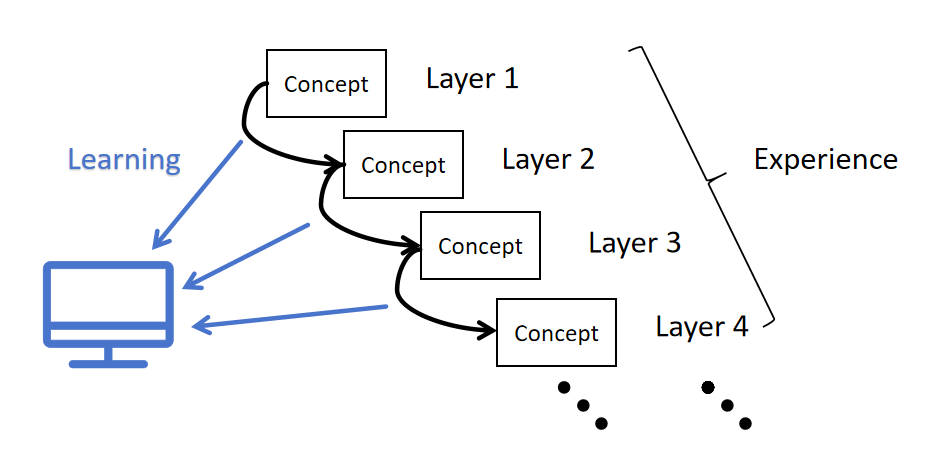
\includegraphics[width=0.9\linewidth]{example_images/ConceptDL}
		\caption{Computer learns from the hierarchical structure of concepts}
		\label{Computer learns from the hierarchical structure of concepts}
	  \end{figure}
    The more layers the structure has, the deeper concepts the computer can learn. After the learning, computers can predict phenomenon and make decisions 
    based on what they have learned. The high-level schematic could be summarized in \autoref{The high-level schematic of deep learning}. The phenomenon or object 
    of interests is the input of the deep learning model. Some simple features will be extracted through sensors, for example the image of the wire harness is extracted 
    through RGB-Camera. The following deep neural network(DNN) can extract more abstract features from the simple features and the computer learns the relations between 
    the features after different layers. After the DNN, the further extracted abstract features should be mapped to the output.  
    \begin{figure}
      \centering
      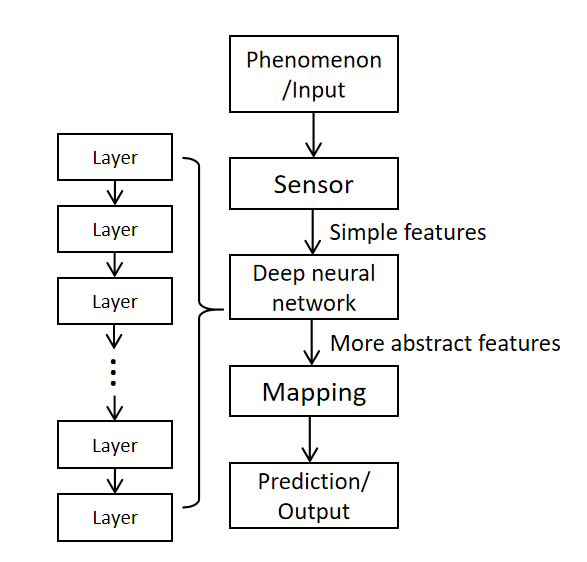
\includegraphics[width=0.6\linewidth]{example_images/DeepLearningSchematic}
      \caption{The high-level schematic of deep learning}
      \label{The high-level schematic of deep learning}
    \end{figure}
  \subsection{Dense neural networks}
  The basic principles of how deep learning works were clarified in the previous section. The next questions are: what is the layer? How does it work to extract features?\\
  In order to answer these two questions more intuitively, the simplest neural network architecture, Dense Neural Network (DNN)\cite{inproceedings}, should be introduced firstly. 
  The DNN simulates the activities of the human brain, which is composed of multiple layers. There could be many neurons in each layer, and all of them are fully connected to 
  all the neurons in the previous layer, see \autoref{Dense neural network}
  The input of the first dense layer is defined as $x_{0}$ and it is also the simple input feature of the network. And the next extracted abstract features are defined as $x_{l}$, 
  where l presents the level of the layer, see \autoref{Mathematical explanation of the feature extraction by layers}.
  The layers are actually defined as some first-order linear mathematical expressions $L _{l}$ with the nonlinear activation function $\Phi_{l}$ in \autoref{eq:layer}, 
  where $w$ is the weight and $b$ is the bias. The nonlinear activation function is important. Without it, the output could be just represented from input by one single layer linearly,
  which is not enough to learn the most of the concepts in the world. Some activation functions are explained in \cite{0706bf17a845490688ef4d7d19df65ba}, e.g., ReLU in \autoref{eq:ReLU}, 
  Sigmoid in \autoref{eq:Sigmoid}, Softmax in \autoref{eq:softmax}. The final step of Schematic, Mapping, can actually be regarded as a layer, which has different options depending on 
  the specific task. For example, for classification, the output layer could be softmax, because it maps the features to probabilities. 
  \begin{figure}
    \centering
    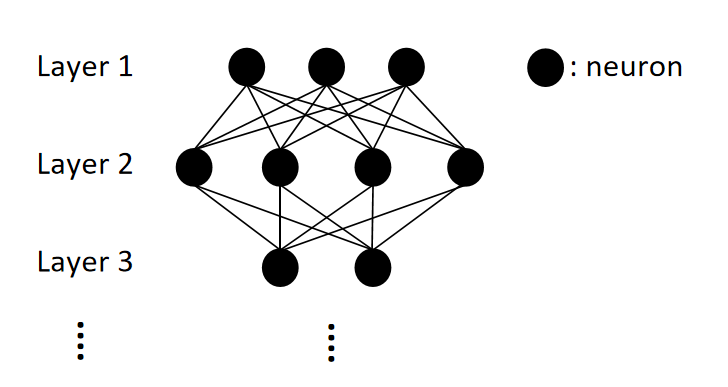
\includegraphics[width=0.6\linewidth]{example_images/DNN}
    \caption{Dense neural network}
    \label{Dense neural network}
  \end{figure}
  \begin{figure}
    \centering
    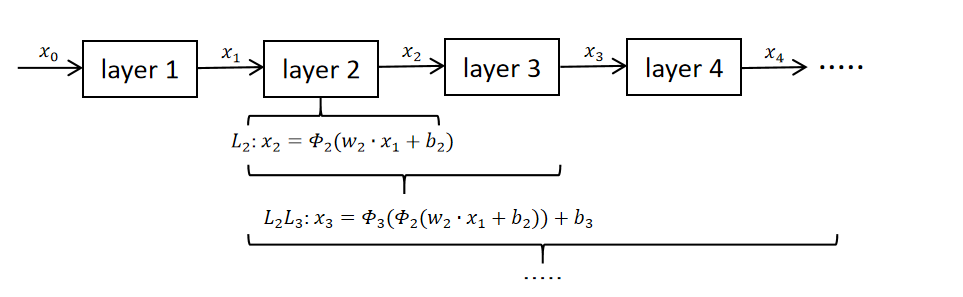
\includegraphics[width=0.9\linewidth]{example_images/mathLayers}
    \caption{Mathematical explanation of the feature extraction by layers}
    \label{Mathematical explanation of the feature extraction by layers}
  \end{figure}
  \begin{align}
    x_{l}=\Phi _{l}(w_{l} \cdot x_{l-1}+ b_{l-1})
     \label{eq:layer}
  \end{align}

  \begin{align}
    \Phi(x) = \begin{cases}
      x& \text{ if } x\ge 0 \\
      0& \text{ else } 
    \end{cases}
     \label{eq:ReLU}
  \end{align}

  \begin{align}
    \Phi(x) = \frac{1}{1+exp(x)^{-1}}  
     \label{eq:Sigmoid}
  \end{align}

  \begin{align}
    \Phi(x_{i}) = \frac{exp(x_{i})}{\sum_{j}exp(x_{j}) } 
     \label{eq:softmax}
  \end{align}
  \subsection{Optimization through backpropagation}
  So far, the process of how initial simple features are extracted and transformed step by step into deeper features through different layers and finally mapped into outputs, 
  i.e., predictions, has been well explained. Then a further question follows: how do networks make accurate predictions?\\
  The transformations and mapping are basically performed by \autoref{eq:layer}. Its result is determined by the activation function $\Phi$, weights $w$ and bias $b$. 
  A GroundTruth $y^{\star }$ needs to be artificially introduced to guide the network to learn the correct behavior, i.e. to predict the desired output. This is explained as
  learning from examples in \cite{russel2010}, which is also well-known as supervised learning. \\
  The prediction of the model or the output after mapping is defined as $y$. A Loss function could be derived. y is actually the result of Mapping, which is actually the output 
  of activation function $\Phi(x)$. It can be further backpropagated onto the feutures from last layer. The optimal weight $w^{star}$ and bais $b^{star}$ are obtained by 
  minimizing the loss equation, see \autoref{eq:Optimization by loss function}. 
  \begin{align}
    w_{l-1}^{\star}, b_{l-1}^{\star}=arg\min_{w_{l-1},b_{l-1}}(\Phi_{l}(\Phi_{l-1}(w_{l-1}\cdot x_{l-1}+b_{l-1}))-y^{\star } ) 
     \label{eq:Optimization by loss function}
  \end{align}
  This approach of optimization can be backwards until the weights and bias of all Layers in the network have been optimized and updated. The whole process is illustrated in 
  \autoref{Parameters are optimized by backpropagation}.
  \begin{figure}
    \centering
    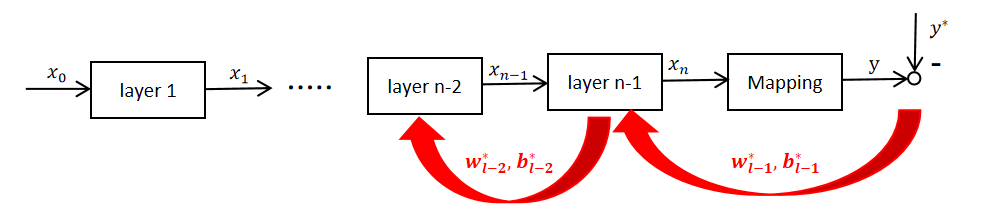
\includegraphics[width=0.9\linewidth]{example_images/bachpropagation}
    \caption{Parameters are optimized by backpropagation}
    \label{Parameters are optimized by backpropagation}
  \end{figure}
  \subsection{Loss Function}
  The loss function in deep learning describes the difference between the groundtruth and the predicted output. The model parameters are optimized and updated by minimizing 
  this function and backpropagating. The loss function could be minimized because it has a gradient $G$. In \autoref{The loss decreases along the direction of the gradient},
  $\theta$ is the model parameter, such as weight, bias. If the gradient is so small, then the loss is difficult to converge. Or if it is so big, then the loss changes oscillatory.
  Hence, a proper loss function is important for deep learning. 
  \begin{figure}
    \centering
    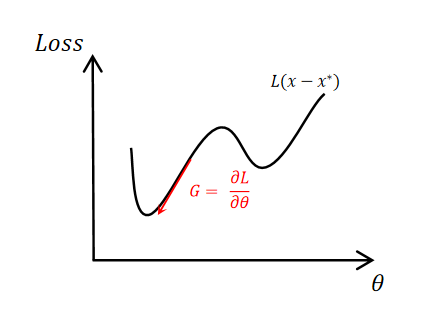
\includegraphics[width=0.6\linewidth]{example_images/loss function}
    \caption{The loss decreases along the direction of the gradient $G$}
    \label{The loss decreases along the direction of the gradient}
  \end{figure}
  For example, l1 in \autoref{eq:l1 loss} and l2-loss function in \autoref{eq:l2 loss} are widely used for regression tasks.
  \begin{align}
    l_1=\sum_{i=1}^{n} \left | y-y^{\star} \right |  
     \label{eq:l1 loss}
  \end{align}
  \begin{align}
    l_2=\sum_{i=1}^{n}(y-y^{\star})^2
     \label{eq:l2 loss}
  \end{align}
  In contrast to the l1-loss function, which is not differentiable at zero, l2 is more often chosen as the loss function because the l2 loss equation is differentiable everywhere.
  But there is also a drawback of l2-loss. When there is an unusual data, the l2 loss will become huge due to squaring. It will affect the training. So the choice of loss function 
  needs to be considered depending on different situations, and sometimes it is necessary to test the effect of different loss functions by doing experiments. In \cite{Sun_2018_ECCV},
  they experimented both l1 and l2-loss for the joint regression task and found that l1-loss function worked consistently better than l2-loss function.\\
  Some other loss functions for segmentation tasks are also introduced in \cite{azad2023loss}. Cross Entropy(CE) loss, in \autoref{eq:CE loss}, is used to the difference between two
  probability distributions. $y^{\star}$ is a one-hot encoded vector and only the targets will be considered.
  \begin{align}
    L_{CE}(y,t) = -\sum_{i=1}^{n} y^{\star} \cdot log(y_{i})
     \label{eq:CE loss}
  \end{align}
  \subsection{Hyperparameter}
  In contrast to the model parameters, hyperparameters cannot be optimized at the backpropagation, but they affect the performance of the model in the meantime as well. 
  In \cite{4e568dfccc734aa6a8184f781bac6353}, the hyperparameters are divided into two groups: (1) performance-oriented parameters, which could influence the system's processing
  throughout, such as the number of threads working simultaneously, i.e., number of workers. (2) accuracy-oriented parameters, which could influence the accuracy of the training, e.g.,
  learning rate and drop out probabilities. There is an overlap between these two groups, and some parameters will affect them both, such as the batch size.\\
  Proper hyperparameters are very important for the training, which significantly affects the accuracy and system performance of the model. And tuning hyperparameters requires experience 
  and patience from researchers, because there might be trade-off between some parameters, for example in \autoref{Trade-off between batch size}, When the batch size increases, the 
  accuracy of the model increases and the system performance decreases.
  \begin{figure}
    \centering
    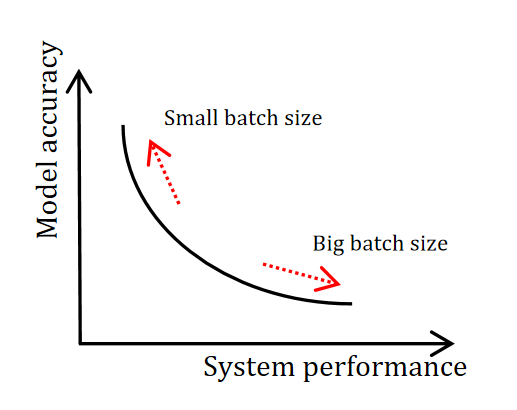
\includegraphics[width=0.6\linewidth]{example_images/batchSize}
    \caption{Trade-off between batch size}
    \label{Trade-off between batch size}
  \end{figure}
  \subsection{Performance metrics}
  Metrics in deep learning are used to measure the performance of a model. Different tasks require different metrics for evaluating. In this subsection, the commonly used metrics 
  will be presented depending on the different specific task.
  \subsubsection{Classification}
  Two states $H_1$ and $H_2$ are going to be classified, $H_1$ represents the positive state and  $H_2$ represents the negative state. The predicted state is defined as $\hat{H}$.
  Then there are four basic metrics to evaluate the model performance, which are True Positive(TP), False Positive(FP), False Positive(FP) and False Negative(FN).
  The cases they correspond to are shown in \autoref{Four basic metrics for classification}.
  \begin{figure}
    \centering
    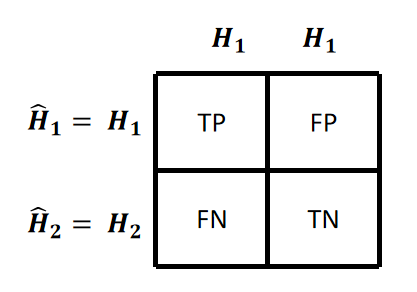
\includegraphics[width=0.6\linewidth]{example_images/basicMetrics}
    \caption{Four basic metrics for classification}
    \label{Four basic metrics for classification}
  \end{figure}
  Then three metrics that are widely used in classification tasks can be derived: \textbf{Accuracy} in \autoref{eq:Accuracy} means the percentage of correctly classified data
  out of the total number of data. \textbf{Precision} in \autoref{eq:Precision} means the percentage of positive data out of the all data predicted to be positive. 
  \textbf{Recall} in \autoref{eq:Recall} means the percentage of correctly predicted positive data out of the all actual positive data.
  \begin{equation}
    \begin{aligned}
      Accuracy = \frac{TP + TN}{TP + TN + FP + FN}
        \label{eq:Accuracy}
    \end{aligned}
  \end{equation}
  \begin{equation}
    \begin{aligned}
      Precision = \frac{TP}{TP + FP}
        \label{eq:Precision}
    \end{aligned}
  \end{equation}
  \begin{equation}
    \begin{aligned}
      Recall = \frac{TP}{TP + FN}
        \label{eq:Recall}
    \end{aligned}
  \end{equation}
\subsubsection{Regression}
The Metrics for regression tasks are similar to its loss functions. For example, Mean Squared Error(MSE) in \autoref{eq:MSEmetrics} and Mean Absolute Error(MAE)
in \autoref{eq:MAEmetrics} could either be used as the loss function as the metrics for evaluation. 
\begin{equation}
  \begin{aligned}
    MSE = \frac{1}{n} \sum_{i=1}^n (\hat{y}_i - y_i)^2
      \label{eq:MSEmetrics}
  \end{aligned}
\end{equation}
\begin{equation}
  \begin{aligned}
    MAE = \frac{1}{n} \sum_{i=1}^n |\hat{y}_i - y_i|
      \label{eq:MAEmetrics}
  \end{aligned}
\end{equation}
\subsubsection{Keypoint detection}
Object Keypoint Similarity (OKS) is a metric used to evaluate the accuracy of keypoint detection. In \cite{Maji_2022_CVPR}, the author introduced it as \autoref{eq:OKS},
which is for each keypoint individually.
\begin{equation}
  \begin{aligned}
    OKS = \frac{\sum_{i=1}^{K} \exp \left( -\frac{d_i^2}{2s^2k_i^2} \right) \cdot \delta(v_i > 0)}{\sum_{i=1}^{K} \delta(v_i > 0)}
      \label{eq:OKS}
  \end{aligned}
\end{equation}
Where:
\begin{itemize}
    \item \( d_i \) is the Euclidean distance between the predicted keypoint and the ground truth keypoint.
    \item \( s \) is scale of the object, e.g., the size of the bounding box.
    \item \( k_i \) is the keypoint specific weight.
    \item \( v_i \) is the visibility flag, e.g., 0 for not labeled and not visible keypoints, 1 for labeled but not visible keypoints, 2 for labeled and visible keypoints.
\end{itemize}
\section{Convolutional neural network}
  DNN can extract very deep features by connecting multiple layers. But Yann LeCun in \cite{LeCun1995-LECCNF} also pointed out some drawbacks:
  \begin{itemize}
    \item [1)] The number of parameters is huge and grows quadratically with the number of neurons per layer, which could lead to the problems like overfitting and memories.
    \item [2)] The topology of the input is entirely ignored and it is not suitable to learn global features due to the full connections of neurons. But the image 
    has a strong 2D local structure. Therefore, images are also not suitable as inputs to DNN.
  \end{itemize}
  Convolutional neural network(CNN) doesn't suffer from either of these problems because of the  weight sharing technique and local connectivity. 
  The input is defined as a 2D-image with $C_{l-1}$ channels, length $H_{l-1}$ and width $W_{l-1}$. The convolutional layer is a four dimensional tensor $C_{l-1} \times C_{l} \times K_{l} \times K_{l}$,
  which means it has $C_{l}$ kernels and each kernel has $C_{l-1}$ filters of size $K_{l} \times K_{l}$. Each channel of the input corresponds to a filter of the kernel. All channels corresponding to 
  the sliding window are mapped into a new channel for the output through all filters of a kernel, see \autoref{Convolutional neural network}. The relationship between the size of the output and 
  the size of the input is shown in \autoref{eq:CNN size change}. When extract the deep features of images, the size of the image will be compressed and the number of channels will increase.
  \begin{figure}
    \centering
    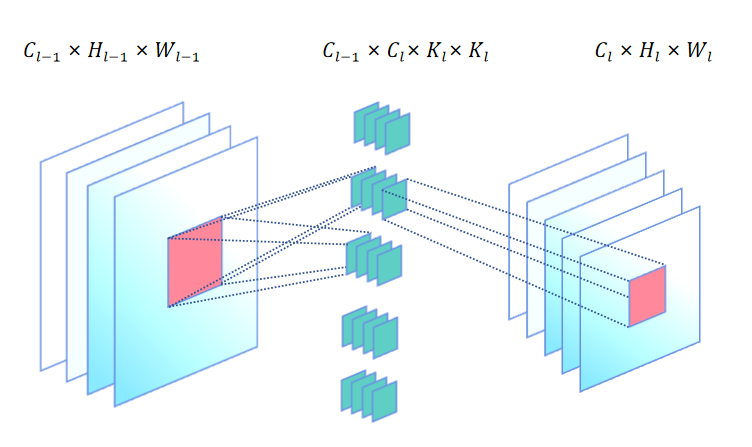
\includegraphics[width=0.9\linewidth]{example_images/CNN}
    \caption{Convolutional neural network}
    \label{Convolutional neural network}
  \end{figure}
  \begin{equation}
  \begin{aligned}
    H_{l}&=H_{l-1}-K_{l}+1\\
    B_{l}&=B_{l-1}-K_{l}+1
      \label{eq:CNN size change}
  \end{aligned}
  \end{equation}
  It is also possible to add modifications to the convolution, such as padding $P$, stride $S$, dialation $D$. When all modifications are included, the size of output image is in \autoref{eq:Modifications} 
  \begin{equation}
  \begin{aligned}
    H_{l}&=\frac{H_{l-1}+2P-(k_{l}-1)D-1}{S}\\
    W_{l}&=\frac{W_{l-1}+2P-(k_{l}-1)D-1}{S}
      \label{eq:Modifications}
  \end{aligned}
  \end{equation}
\section{Transformer}
  In this section, the transformer will be introduced in detail. Think about keypoint detection tasks for the wire harness. The background is regarded as 
  the disturbance. The basic idea is ignoring the non-relevant part and only focusing on the wire harness. 
  The original model architecture of the transformer is shown in \autoref{The Transformer model architecture}, which is firstly proposed by Vaswani in 2017 \cite{NIPS2017_3f5ee243}. 
  It consists of an encoder and decoder structure. 
  It was initially employed to process natural language processing (NLP) tasks such as text translation and generation. 
\subsection{Attention}
  The input to encoder composes of three parts:
  query(Q), key(K) and value(V). The query can be viewed as the vector form of a word in text. It could correspond to several keys, which represent vectors of the all words 
  in a text. The value represents the extracted information vector from the all words. $Attention(Q, K, v)$ represents the match between each word
  is usually calculated in \autoref{eq:Calculate attention}, where $d_k$ is the dimension of the key vector for avoiding a too large numerator. 
  \begin{equation}
    \begin{aligned}
      Attention(Q,K)=softmax(\frac{Q\cdot K^T}{\sqrt{d_{k}}}) \cdot V 
        \label{eq:Calculate attention}
    \end{aligned}
  \end{equation}
  For example, the score between the words in the sentence "I am a student" are shown in \autoref{Attentions in a sentence}. The four words on a column represent Q, and they each have 4 
  keys. The values in the table grid represent the matches between words. The highest values appear between identical words. The less related the words are to each other, the lower the 
  value. After getting the values between words, it passes through a softmax function, which transforms the values into probabilities between zero and one. Then calculate the dot product
  between the probabilities matrix and the vector V to get the output representation of each word. For easier understanding, the calculation can be expressed as \autoref{Calculate the attentions}.
  \begin{figure}
    \centering
    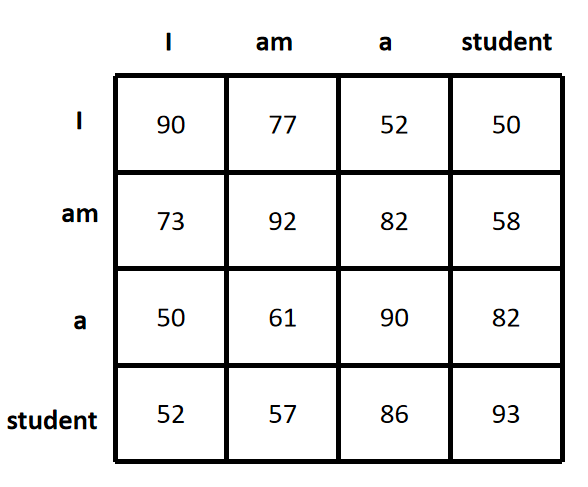
\includegraphics[width=0.6\linewidth]{example_images/IamAStudent}
    \caption{Match between words}
    \label{Attentions in a sentence}
  \end{figure}
  \begin{figure}
    \centering
    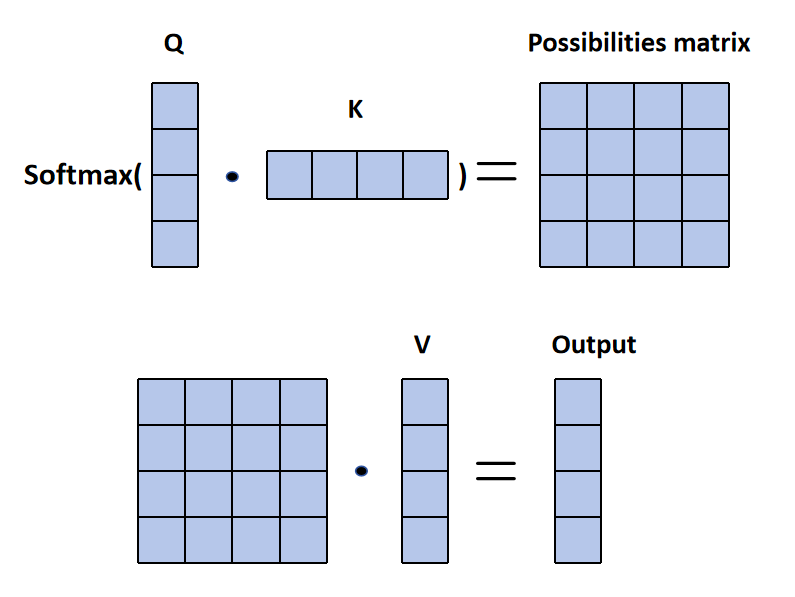
\includegraphics[width=0.6\linewidth]{example_images/AttenCalculation}
    \caption{Calculate the attentions}
    \label{Calculate the attentions}
  \end{figure}
  \begin{figure}
    \centering
    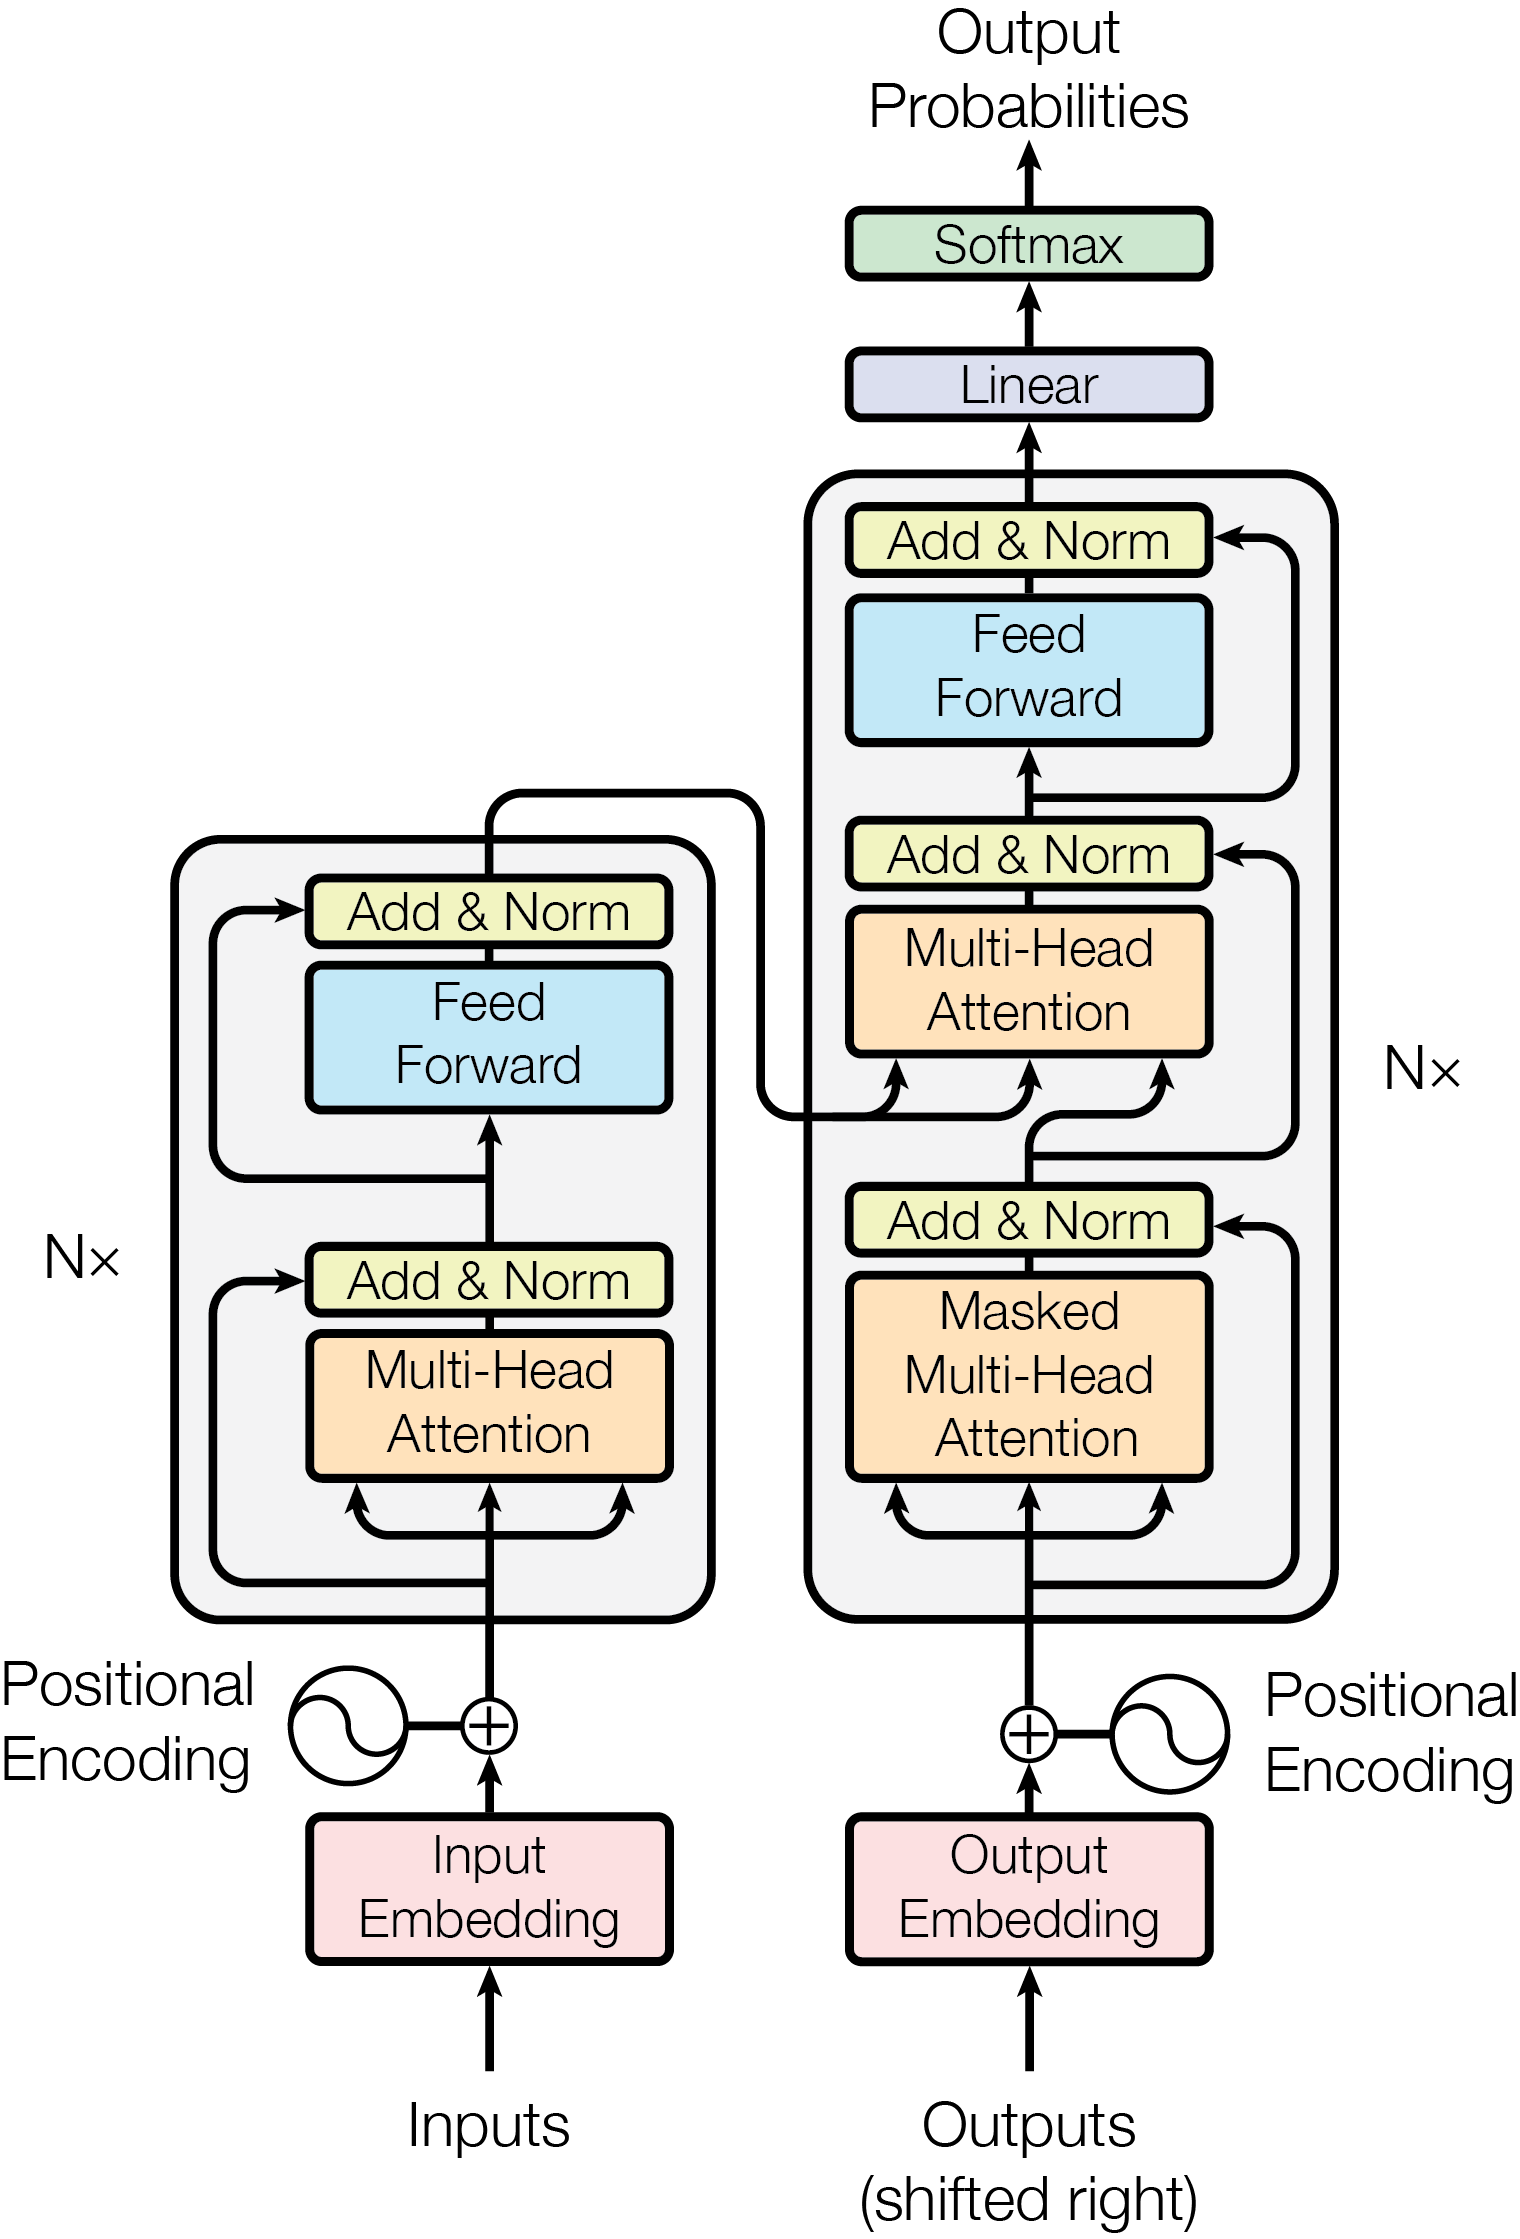
\includegraphics[width=0.6\linewidth]{example_images/transformer}
    \caption{The Transformer model architecture\cite{NIPS2017_3f5ee243}}
    \label{The Transformer model architecture}
  \end{figure}
\subsection{Position Embedding}
  Transformer is unable to understand the sequential relations of  words in the input. So, it is necessary for the model to understand the position of the elements in the sequence.
  The researchers proposed the Position Embedding approach to realize it, which is presented in \autoref{eq:Position Embedding}, where $pos$ is the position of the word in a sentence,
  $d_{model}$ is the dimension of this word vector and $i$ is the indices in the dimension.  After the Position Embedding is obtained, the word vectors are added with it, which are unique
  according to their position information.
  \begin{equation}
    \begin{aligned}
      PE(pos,i) &= sin(\frac{pos}{10000^{2i/d_{model}}})\\
      PE(pos,i+1) &= cos(\frac{pos}{10000^{2i/d_{model}}})
        \label{eq:Position Embedding}
    \end{aligned}
  \end{equation}
\subsection{Mask in decoder}
  The output of encoder will flow into decoder. The purpose of the decoder is to make the model consider the previously generated results when it generates the target sequence.
  The structure of decoder is similar to the encoder. There are two main blocks in decoder. The first block calculates the attention of the generated output and the second 
  block calculates the attention of the encoder's output with the output of the first block in decoder. While in encoder the attentions of the query with each of its keys will be
  calculated and considered, each word of the target sequence should only consider the word before it. The mask, which will be introduced in this subsection, is included to avoid 
  the information leakage. It is actually an upper triangular matrix, as shown in \autoref{Mask in decoder}. It is added with the score matrix of output and the results is shown
  in \autoref{The score matrix added with mask}. Due to the infinite negative score in the added matrix, after the softmax function the possibilities will be zero. In this case,
  the output words are independent on the future words.
  \begin{figure}[htbp]
		\centering
		\begin{subfigure}[b]{0.5\textwidth}
			\centering
			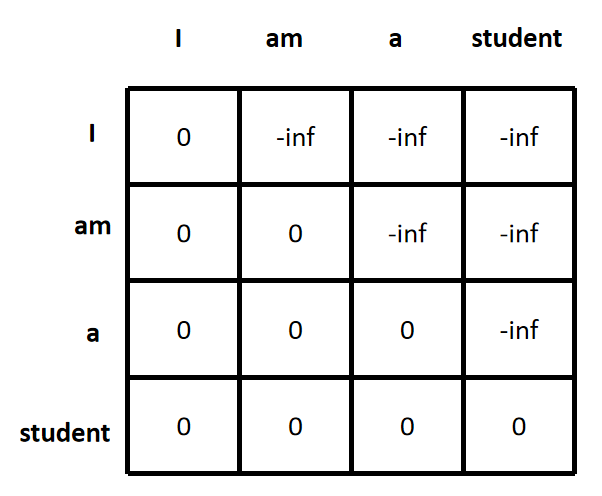
\includegraphics[width=0.9\linewidth]{example_images/mask}
			\caption{Mask in decoder}
			\label{Mask in decoder}
		\end{subfigure}
		\hfill
		\begin{subfigure}[b]{0.5\textwidth}
			\centering
			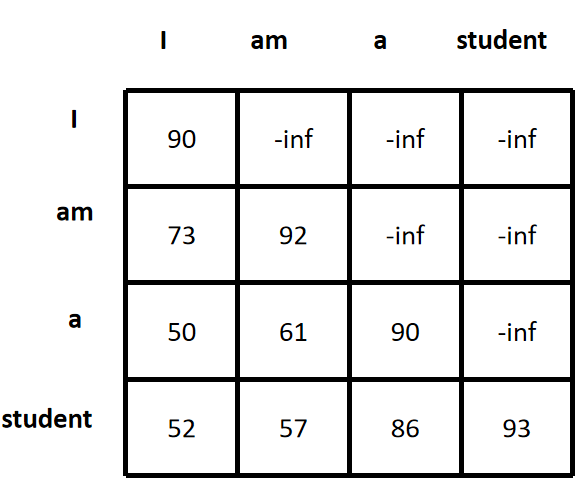
\includegraphics[width=0.9\linewidth]{example_images/mask1}
			\caption{The score matrix added with mask}
			\label{The score matrix added with mask}
		\end{subfigure}
		\caption{Use mask to prevent the influence from future words}
		\label{Use mask to prevent the influence from future words}
	\end{figure}
\subsection{Vision Transformer}
  With the success of Transformer in the field of NLP, researchers began to explore its application in computer vision
\section{Full and individual segment estimation}

\section{Dataset}
    \chapter{Methodology}
In this chapter, the methodologies and tools for preparing the dataset, designing the model and experiment will be introduced. 
\section{Dataset Preparation}
    \subsection{Generate dataset manually}
    The stereo vision camera, fixed on the workbench, is implemented for takes pictures of wire harness \autoref{stereoCamera1}. Once the photograph is completed, the images will be uploaded and stored 
    in the bucket to the database MinIO.
    \begin{figure}
        \centering
        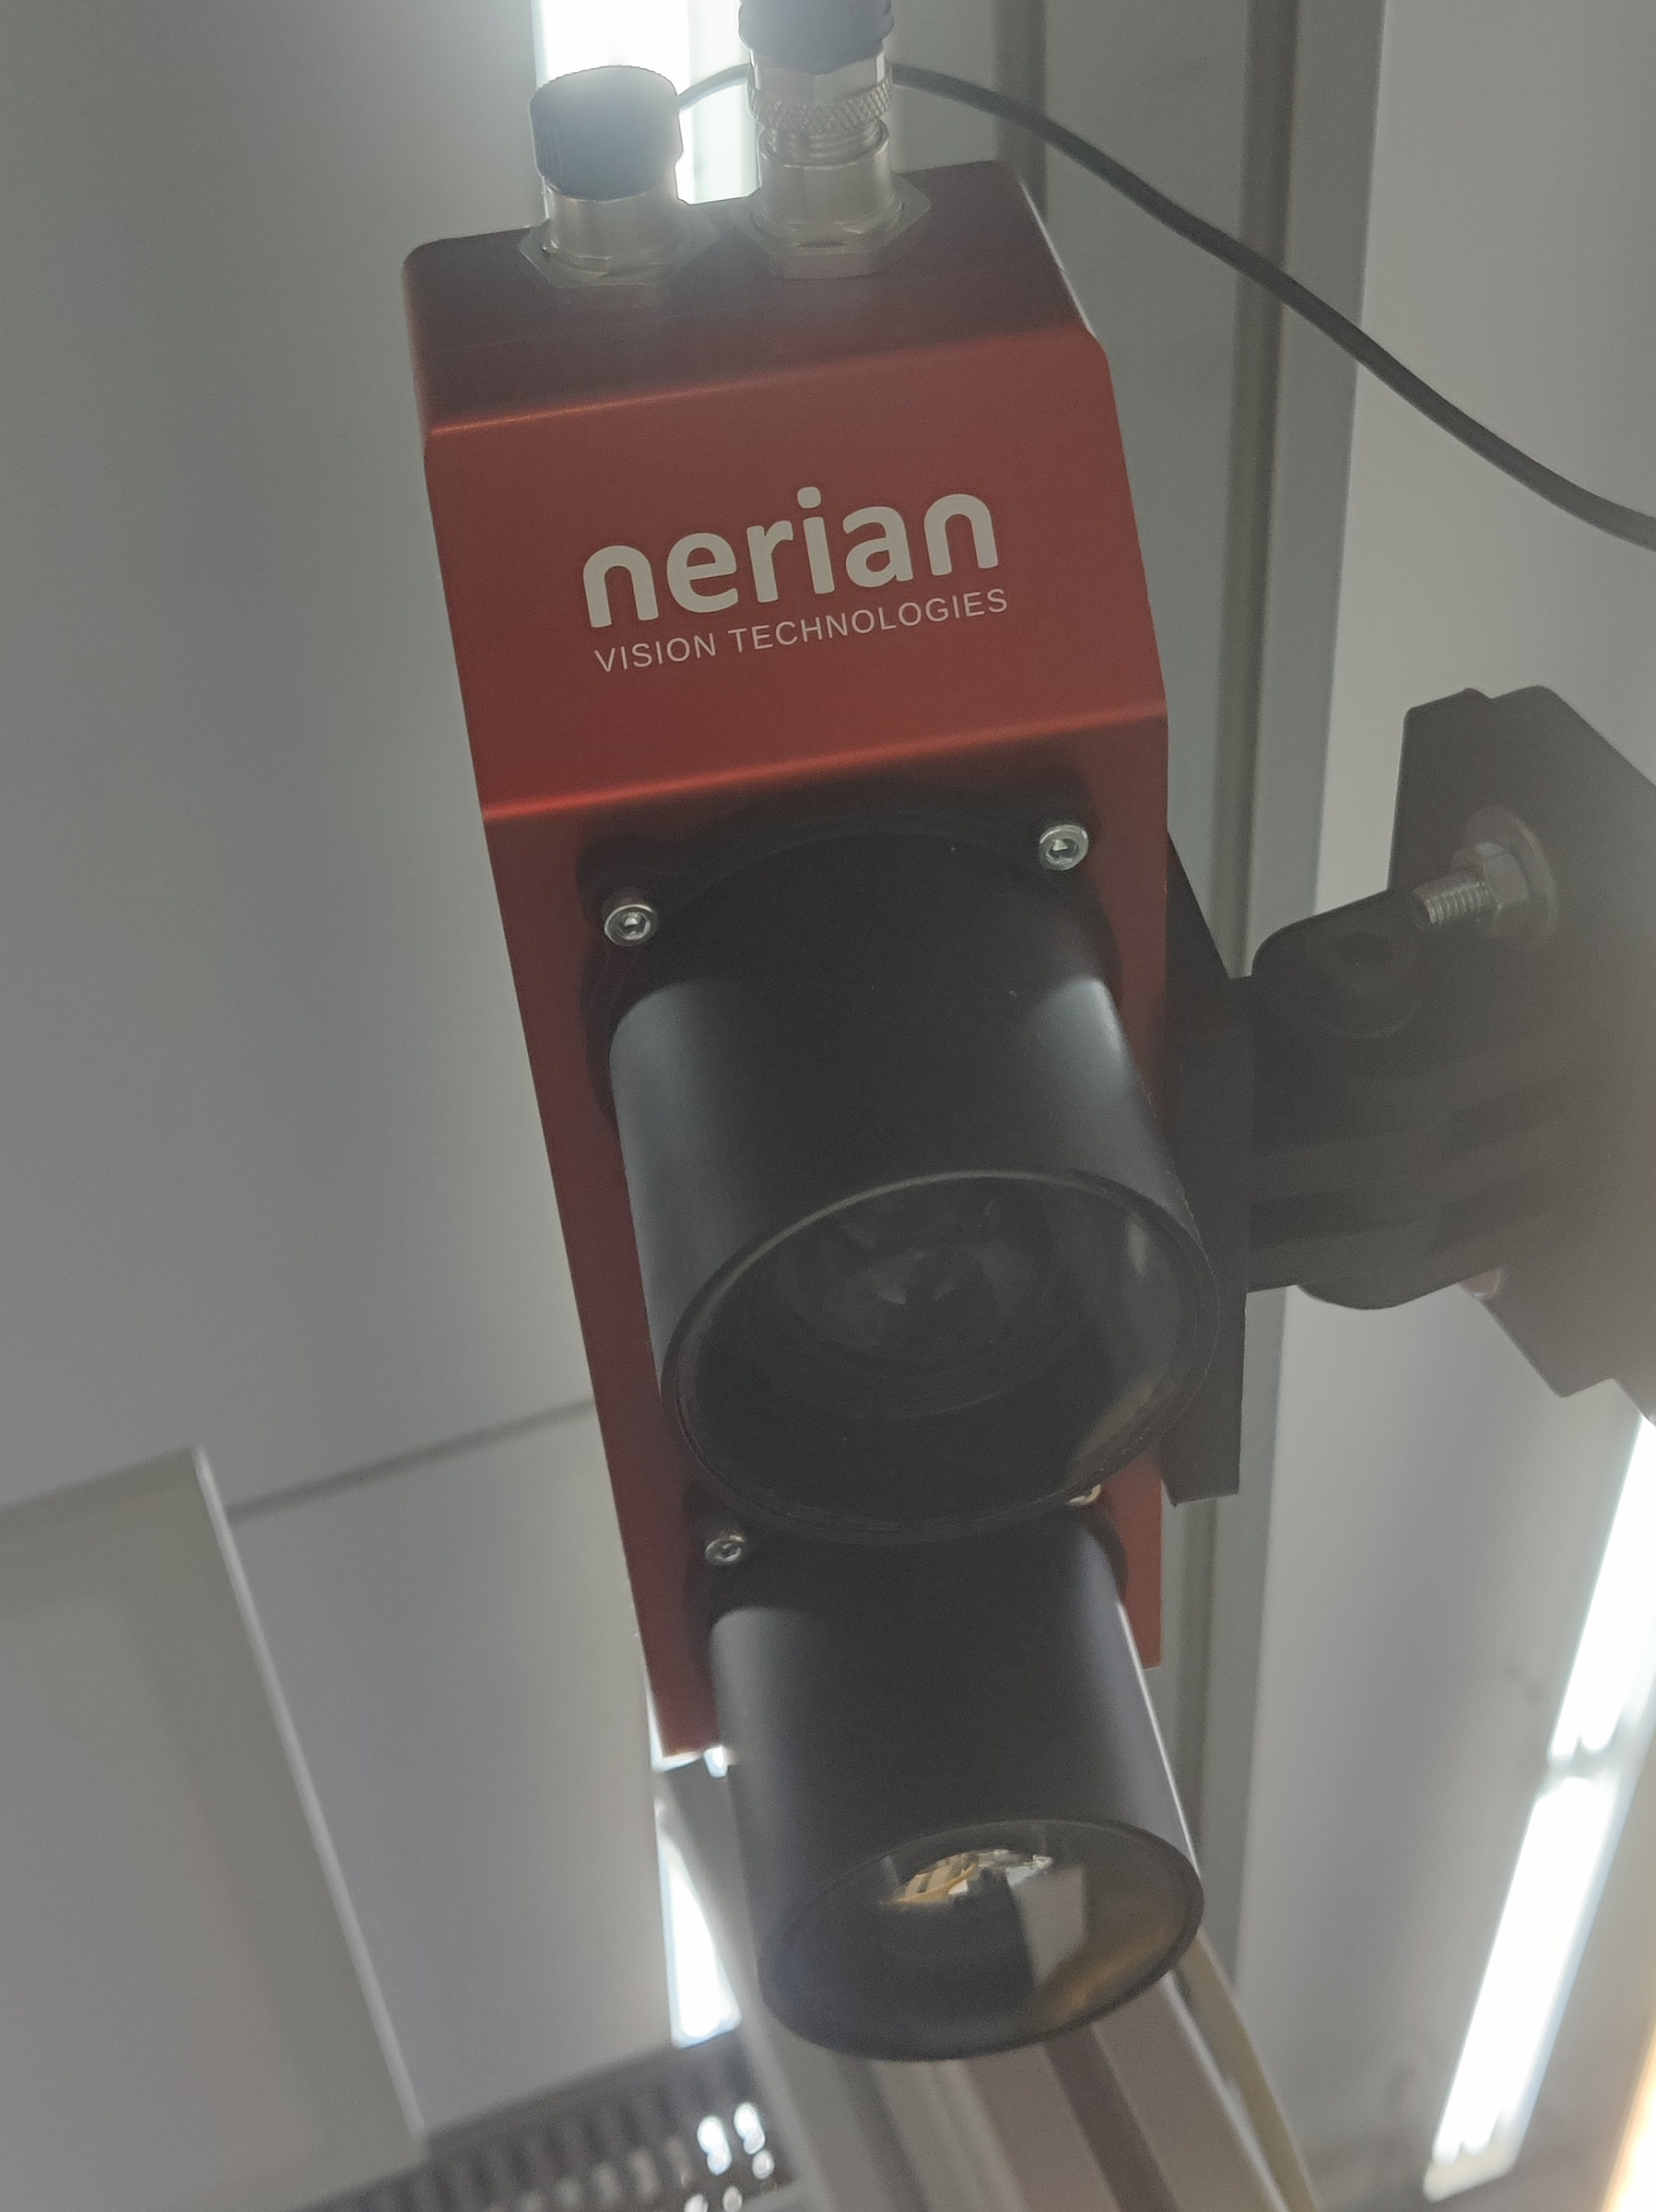
\includegraphics[width=0.4\linewidth]{example_images/stereoCamera1.jpg}
        \caption{Stereo Vision Camera}
        \label{stereoCamera1}
    \end{figure}
    Label studio\cite{LabelStudio} is a popular open-source data labeling tool. It could annotate for different vision tasks, e.g., keypoint detection, object segmentation, image classification.
    Howerver, the goal of this thesis is to construct the spline model of the wire harness by interpolating the keypoints, while the Label studio could only show the annotated keypoints in image.
    An annotation tool is developed through NiceGUI\cite{schindler2024nicegui}, which is a python-based UI framework and will show up in the web browser. The web interface of the annotation tool'
    is shown in \autoref{Annotation tool}. The user could select the bucket in dataset and load the images in this tool. Once the images are loaded, the annotation could begin.
    Click on the segment of the wire harness to create nodes. When there are more than four nodes on the segment, the cubic spline is 
    automatically interpolated. The positions of $n+1$ nodes are defined as $(x_k, y_k)$ for $k = 1, 2, ...n+1$, then the cubic spline between nodes $(x_k, y_k)$ and $(x_{k+1}, y_{k+1})$ is shown in
    \autoref{eq:cubic spline}. The neighboring splines need to fulfill the first and second order boundary conditions in \autoref{eq:boundary conditions}. 
    \begin{equation}
        \begin{aligned}
            &s_k(x) =  c_{k,3}x^3+c_{k,2}x^2+c_{k,1}x+c_{k,0}\\
            &s_k(x_k) = y_k,  s_k(x_{k+1}) = y_{k+1}
            \label{eq:cubic spline}
        \end{aligned}
    \end{equation}
    \begin{equation}
        \begin{aligned}
            s_k'(x_{k+1}) &= s_{k+1}'(x_{k+1})\\
            s_k''(x_{k+1}) &= s_{k+1}''(x_{k+1})
            \label{eq:boundary conditions}
        \end{aligned}
    \end{equation}
    The length and bending energy of the spline are calculated. The spline curve actually consists of numerous points.  The length of the entire spline curve 
    is obtained by summing the Euclidean distances of neighboring discrete points. The algorithm is shown in \autoref{Calculate the length of a spline}.
    \begin{algorithm} 
        \caption{Calculate the length of a spline}
        \label{Calculate the length of a spline}
        \begin{algorithmic}[1]
        \STATE \textbf{Input:} $X$
        \STATE $Length \leftarrow [\quad]$
        \FOR{$(x_{k},y_{k}),(x_{k+1},y_{k+1}) \in X$}
            \STATE $Distance \leftarrow \sqrt{(x_{k+1}-x_{k})^2+(y_{k+1}-y_{k})^2}$
            \STATE $Length.append(Distance)$
        \ENDFOR
        \RETURN $\text{sum}(Length)$
        \end{algorithmic}
    \end{algorithm}
    The benging energy is calcultated as \autoref{eq:bending energy}, where $\kappa(s)$ is the curvature of the spline as a function of the arc length s.
    \begin{equation}
        \begin{aligned}
            E = \int_{0}^{L} \kappa(s)^2ds
            \label{eq:bending energy}
        \end{aligned}
    \end{equation}
    The spline is defined in parametric form as $s(t) = (x(t),y(t))$ and the curvature spline be calculated as \autoref{eq:curvature}. 
    \begin{equation}
        \begin{aligned}
            \kappa(t) = \frac{\dot{x}(t) \ddot{y}(t) - \dot{y}(t) \ddot{x}(t)}{(\dot{x}(t)^2 + \dot{y}(t)^2)^{3/2}}
            \label{eq:curvature}
        \end{aligned}
    \end{equation}
    The whole equation could be represented in discrete form in \autoref{eq:curvature discrete form}.
    \begin{equation}
        \begin{aligned}
            E = \int_{0}^{L} \kappa(s)^2 \, ds = \int_{t_0}^{t_1} \kappa(t)^2 \left( \sqrt{\dot{x}(t)^2 + \dot{y}(t)^2} \right) \, dt
            \label{eq:curvature discrete form}
        \end{aligned}
    \end{equation}
    After one branch is labeled, the user could press up key to start labeling the next segment. The number of nodes on each segment should be the same. The sequences of 
    segments could also be adjusted. This is important for the model to learn the structure of the wire harness when the segments are not sorted in the program or the complexity 
    is too high to sort. Once all the segments are labeled, the annotations could be saved and exported as json file.
    \begin{figure}{!htbp}
        \centering
        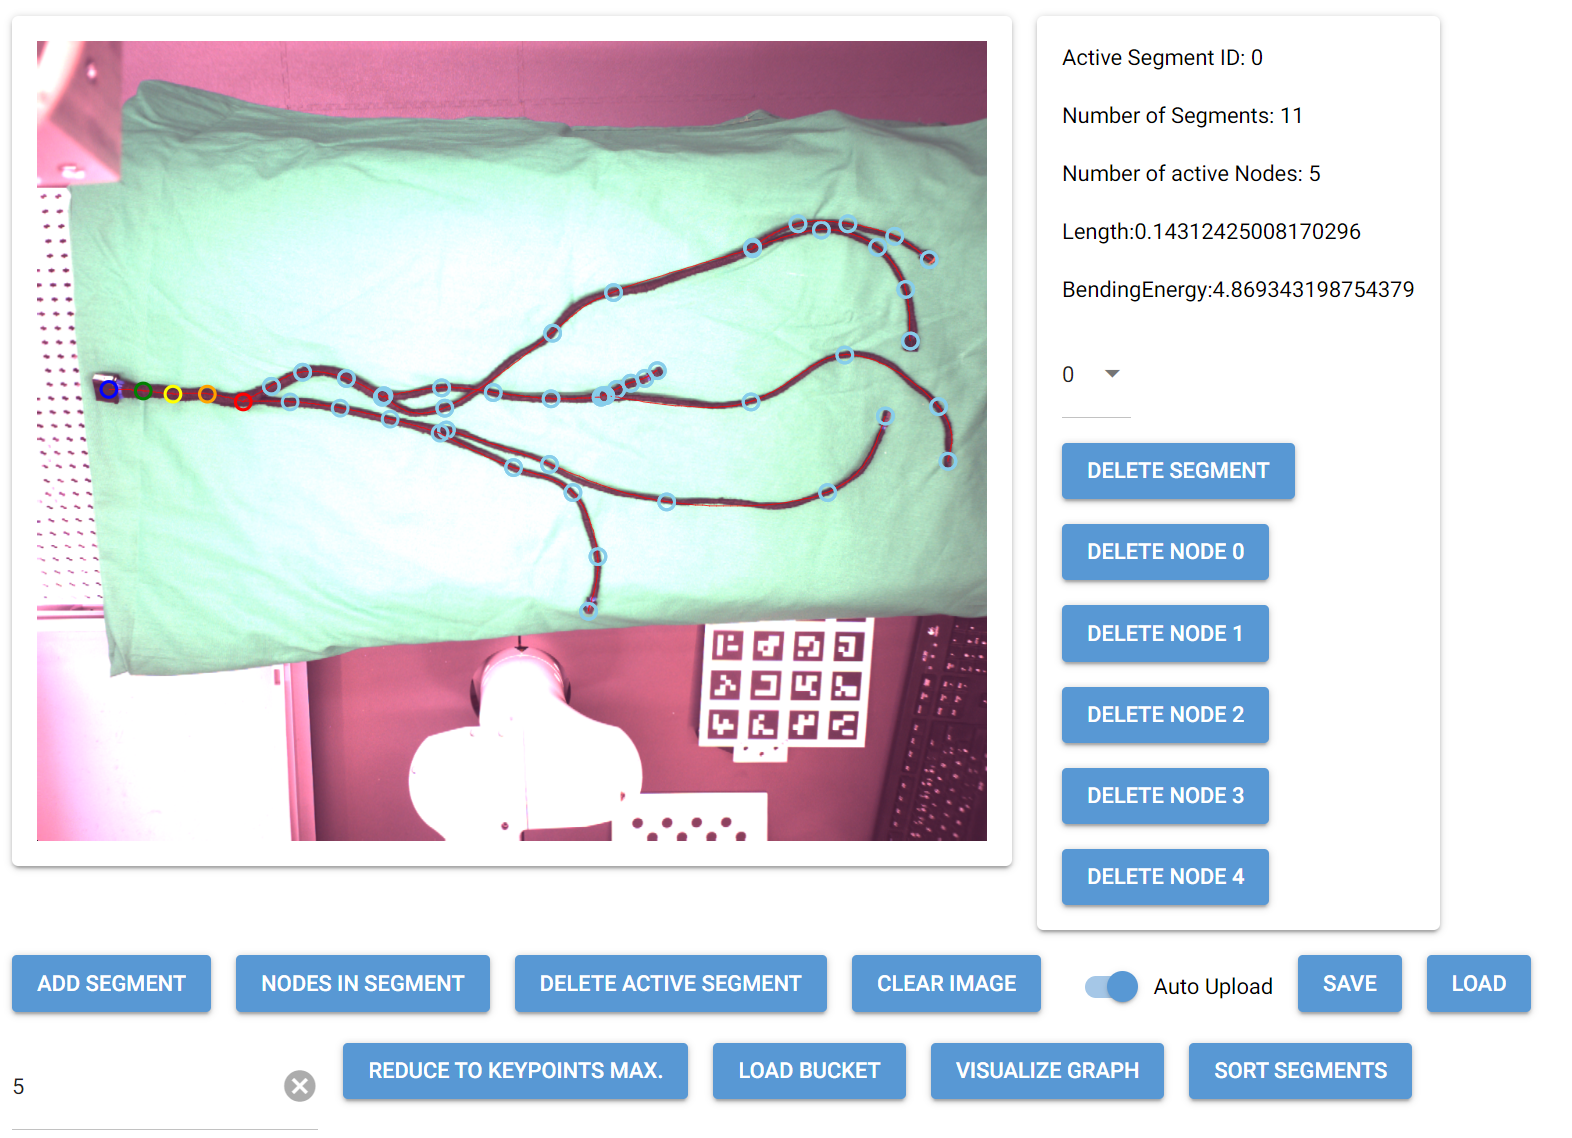
\includegraphics[width=0.9\linewidth]{example_images/NiceGUIInterface.png}
        \caption{Annotation tool}
        \label{Annotation tool}
    \end{figure}
\subsection{Dataset Expansion}
    Last subsection shows the approach of generating the dataset of the wire harness by using stereo vision camera and the annotation tool. However, annotating a large  
    dataset manually is time-consuming and inefficient. A small dataset could lead to the problem of under-fitting and the bad generalization. In this subsection, two 
    developed methods for expanding the datasets are introduced. 
\subsubsection{Synthetic images of BDLOs}
    A synthetic dataset of the eleven-segment wire harnesses is generated for transfer learning, which has the same topology as \autoref{fig:Topology of the eleven-segment wire harness}.
    To set up the configuration, the topology, the number of keypoints and the length of each segment are defined in advance. The cubic spline is obtained by interpolating randomly generated 
    control points under certain constraints, e.g. the maximum angle between two neighboring keypoints is set in \autoref{The constraint of maximum angle between two neighboring keypoints}
    to prevent the interpolating spline from being too curved. 
    \begin{figure}[!htbp]
        \centering
        \includegraphics[width=0.5\linewidth]{example_figures/MaxAngle_synthetic.pdf}
        \caption{The constraint of maximum angle between two neighboring keypoints}
        \label{The constraint of maximum angle between two neighboring keypoints}
    \end{figure}
    To make the fake image a better representation of some special situations such as overlapping, the lighting condition is mimic
    by means of a convolutional kernel to minimize the gap between the real and fake images. From the edges to the center of the segment, the pixel become lighter in color. An example of the 
    synthetic wire harness is shown in \autoref{An example of the synthetic image of the eleven-segment wire harness}.
    \begin{figure}[!htbp]
        \centering
        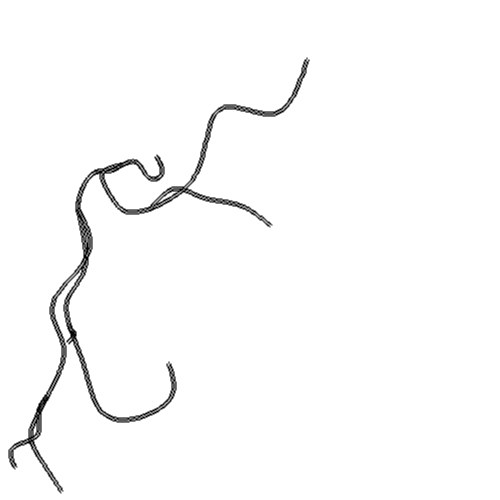
\includegraphics[width=0.4\linewidth]{example_figures/fakeimg.png}
        \caption{An example of the synthetic image of the eleven-segment wire harness}
        \label{An example of the synthetic image of the eleven-segment wire harness}
    \end{figure}
\subsubsection{Operations on segments}
    The dataset could be extended by operations on segments, e.g, rotation and translation. To operate on the branches of the harness, the harness 
    first needs to be segmented. Here the images are firstly segmented to individual segments by using Label-Studio, see \autoref{fig:Wire Segmentation}.\\
	\begin{figure}[!htbp]
		\centering
		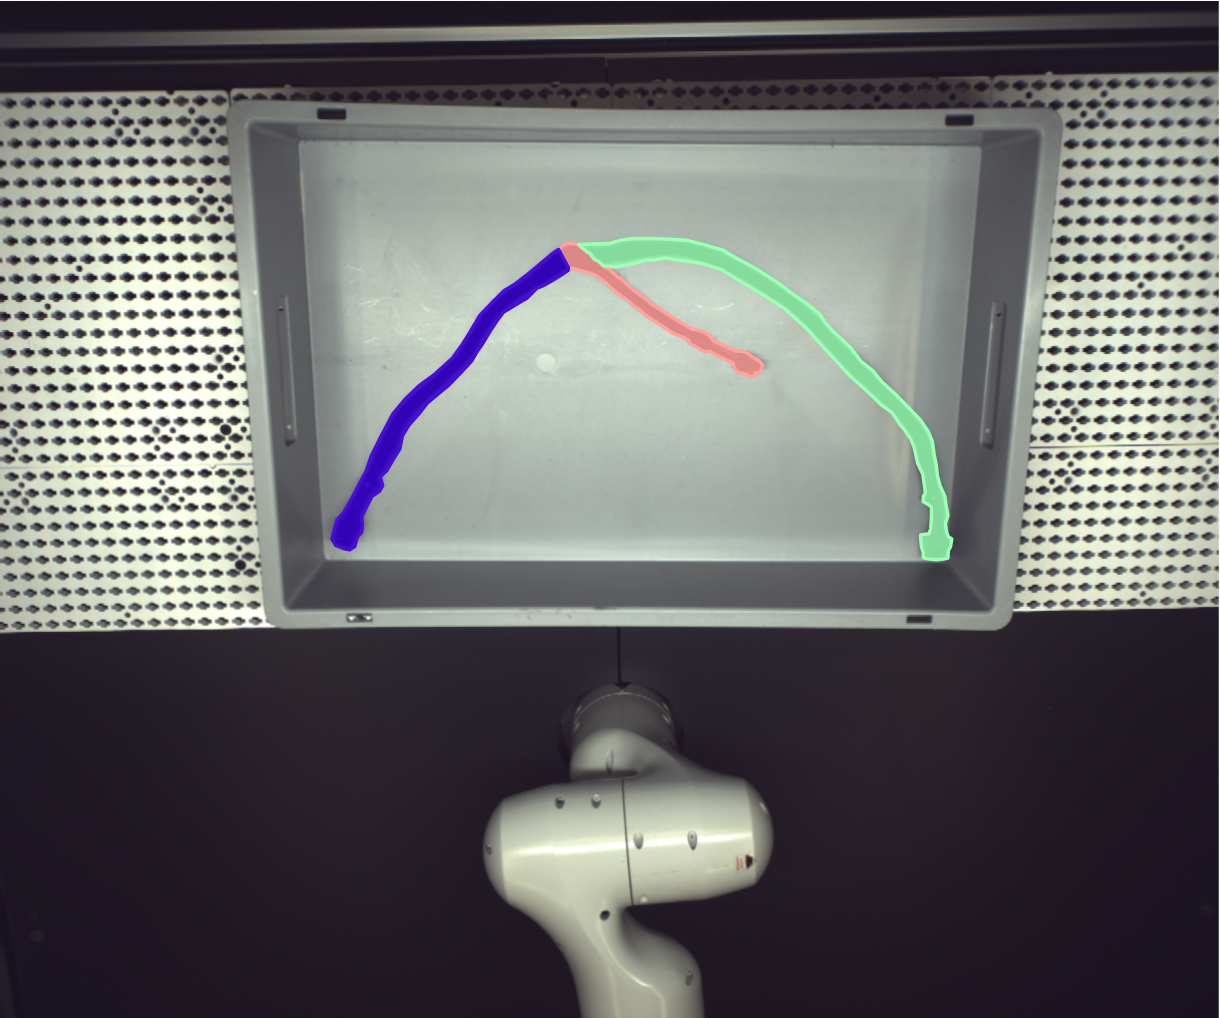
\includegraphics[width=0.6\linewidth]{example_images/img_0_segment}
		\caption{Wire Segmentation}
		\label{fig:Wire Segmentation}
	\end{figure}
	A rotation matrix is defined as \autoref{eq:rotation matrix}:
	\begin{align}
		\begin{bmatrix}
			cos(\theta)&  -sin(\theta )&x \\
			sin(\theta )&  cos(\theta )&y  \\
			0&  0&1
		\end{bmatrix} \label{eq:rotation matrix}
	\end{align}
	An all-zeros mask will be created firstly that has the same size as the image of wire harnesses. The values on mask, where corresponds to the coordinate position of
	annotated points of segmentation, are then equal to one. The corresponding image region $\mho$ of the wire harness will be segmented as a polygonal region based on the mask.
	Build the rotation matrix relative to the desired position and then calculate its corresponding new coordinates by using \autoref{eq:new region}. 
	Paste the previously segmented polygonal area onto the empty background. The new generated virtual image is \autoref{fig:fake image}.
	\begin{align}
		\mho ^{\star } = \mho \cdot \begin{bmatrix}
			cos(\theta)&  -sin(\theta )&x \\
			sin(\theta )&  cos(\theta )&y  \\
			0&  0&1
		\end{bmatrix} \label{eq:new region}
	\end{align}

	\begin{figure}[!htbp]
		\centering
		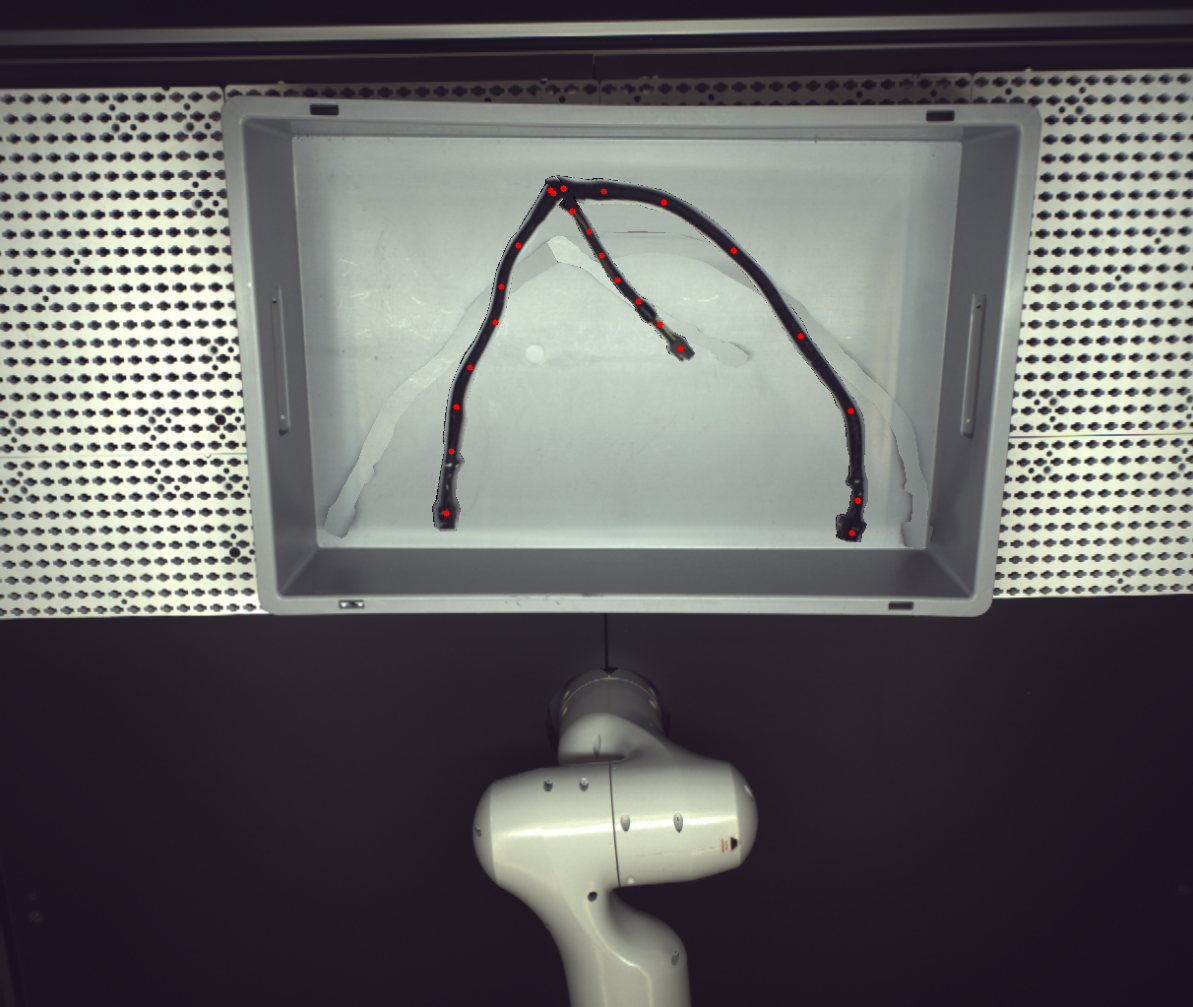
\includegraphics[width=0.6\linewidth]{example_images/img_0_segment_fakeImages}
		\caption{fake image}
		\label{fig:fake image}
	\end{figure}
	The corresponding annotation $\Theta $ could also be calculated with the rotation matrix as \autoref{eq:new anno}:
	\begin{align}
		\Theta ^{\star } = \Theta \cdot \begin{bmatrix}
			cos(\theta)&  -sin(\theta )&x \\
			sin(\theta )&  cos(\theta )&y  \\
			0&  0&1
		\end{bmatrix} \label{eq:new anno}
	\end{align}
\section{Model}
\section{Experiment}
    \chapter{Experiment}
This chapter begins by the experiment of simple three-branched wire harness for fast verification of key points detection methodology.
Followed by the experiment of wire harness with more branches to validate the feasibility in industry.
\section{Three branched wire harness}
In this section, the dataset used for training, generated model and the training's configuration and results will be introduced.
\subsection{Dataset}
The dataset consists of 100 images of three branched wire harnesses, see \autoref{fig:Three branched wire harness}. The dataset is split to 
two parts, 80 images for training and 20 images for validation.
In annotation,there are eight key points for each segment, which could be interpolated by cubic spline and formed as the wire spline model.
\begin{figure}[htbp]
    \centering
    \begin{subfigure}[b]{0.45\textwidth}
        \centering
        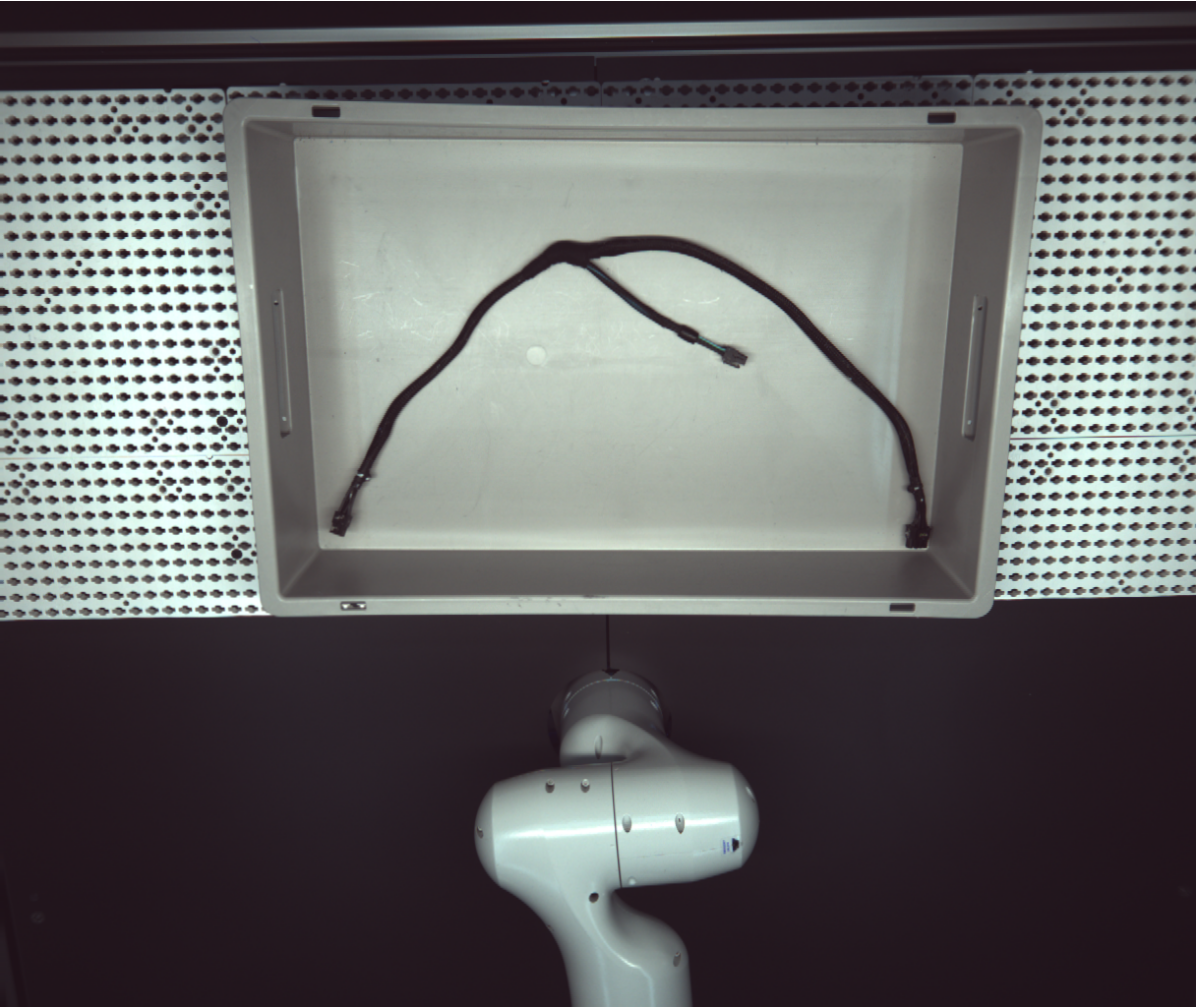
\includegraphics[width=0.9\linewidth]{example_images/img_0}
        \caption{Three branched wire harness without annotation}
        \label{fig:Three branched wire harness original}
    \end{subfigure}
    \hfill
    \begin{subfigure}[b]{0.45\textwidth}
        \centering
        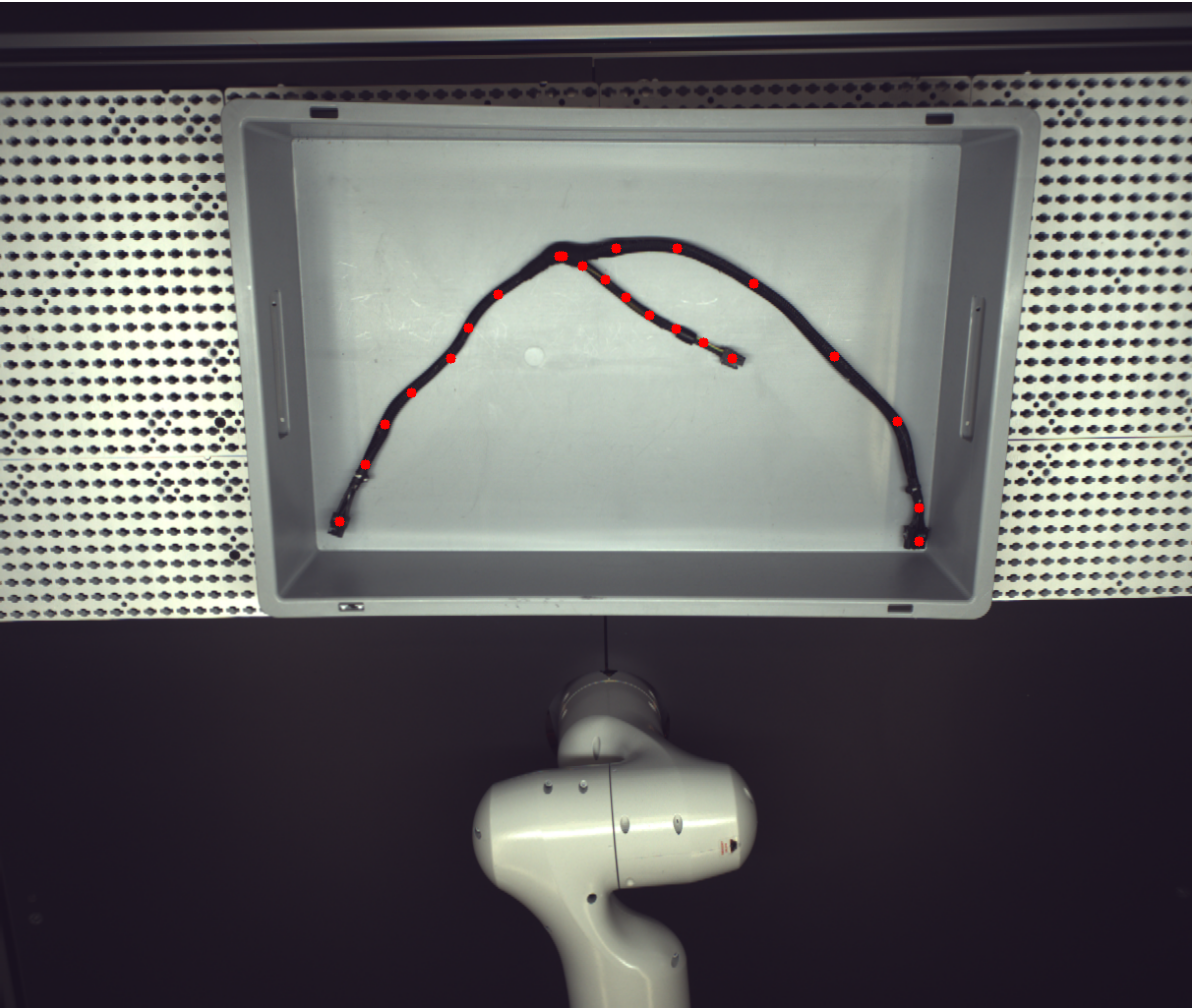
\includegraphics[width=0.9\linewidth]{example_images/img_0_anno}
        \caption{Three branched wire harness with annotation}
        \label{fig:Three branched wire harness with annotation}
    \end{subfigure}
    
    \caption{Three branched wire harness}
    \label{fig:Three branched wire harness}
\end{figure}
\subsection{Model}
The Model are composed of three parts: backbone, neck and head.\\
For this task, the Swin-Transformer is employed as backbone. After the backbone, features are extracted and the dimension of input image changes 
from 1x3x256x256 to 1x768x32x32. The image has a smaller size but deeper features.
Between them, there are also two stages and the feature dimensions are 192 and 384, respectively. 
The four stages will then be collected to feed into the neck, Feature Pyramid Networks. The output tensor of the FPN is upsampled in head by using
Transposed Convolution to reconstruct to task-specific dimensions.
In this case is 1x3x8x256x256, which means 3 segments, 8 key points and the image size is 256x256.
\subsection{Training} 
The model is trained with SGD optimizer and the batch size is 2. After 106 epochs, the loss will end with 1.28, see \autoref{fig:Training result}.\\
\begin{figure}
	\centering
	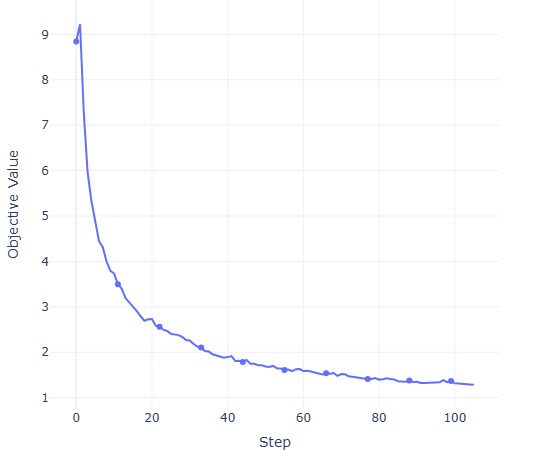
\includegraphics[width=0.6\linewidth]{example_images/noAttn_keypoints_100}
	\caption{Training results}
	\label{fig:Training result}
\end{figure}
The evaluated result is in \autoref{fig:Training result validation}. The result is not ideal, since several keypoints are incorrectly or
inaccurately detected, i.e., detected on the other segment, or outside the wire harnesses. The sequence of keypoints is also not correctly 
ordered, such that the interpolated spline looks not promising. Hence, the model should be optimized.
\begin{figure}
	\centering
	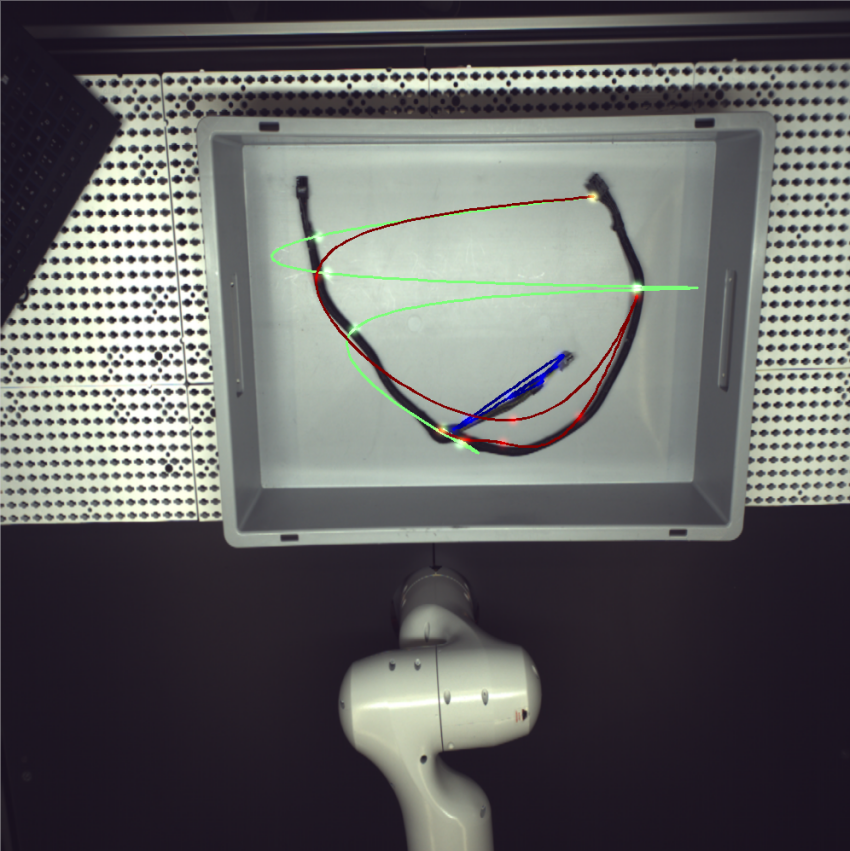
\includegraphics[width=0.6\linewidth]{example_images/noAttn_keypoints_100_eval}
	\caption{Validation}
	\label{fig:Training result validation}
\end{figure}
\subsection{Optimization}
\subsubsection{Self attention}
Since there are several keypoints are detected on the wrong segment. The attentional mechanism might could facilitate the model to pay attention 
to the highlights of the image so that the keypoints are correctly detected on the right segment. The encoder layers of transformer are placed in 
head during upsampling. After training the loss is decreased to 0.83 after 234 epochs, see \autoref{fig:Training result with Attention}. 
The evaluation is in \autoref{fig:Training result validation Attention}.\\
\begin{figure}
	\centering
	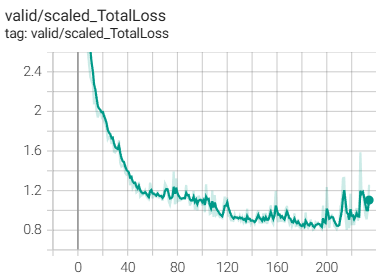
\includegraphics[width=0.6\linewidth]{example_images/withAttn_keypoints_100}
	\caption{Training result}
	\label{fig:Training result with Attention}
\end{figure}
\begin{figure}
	\centering
	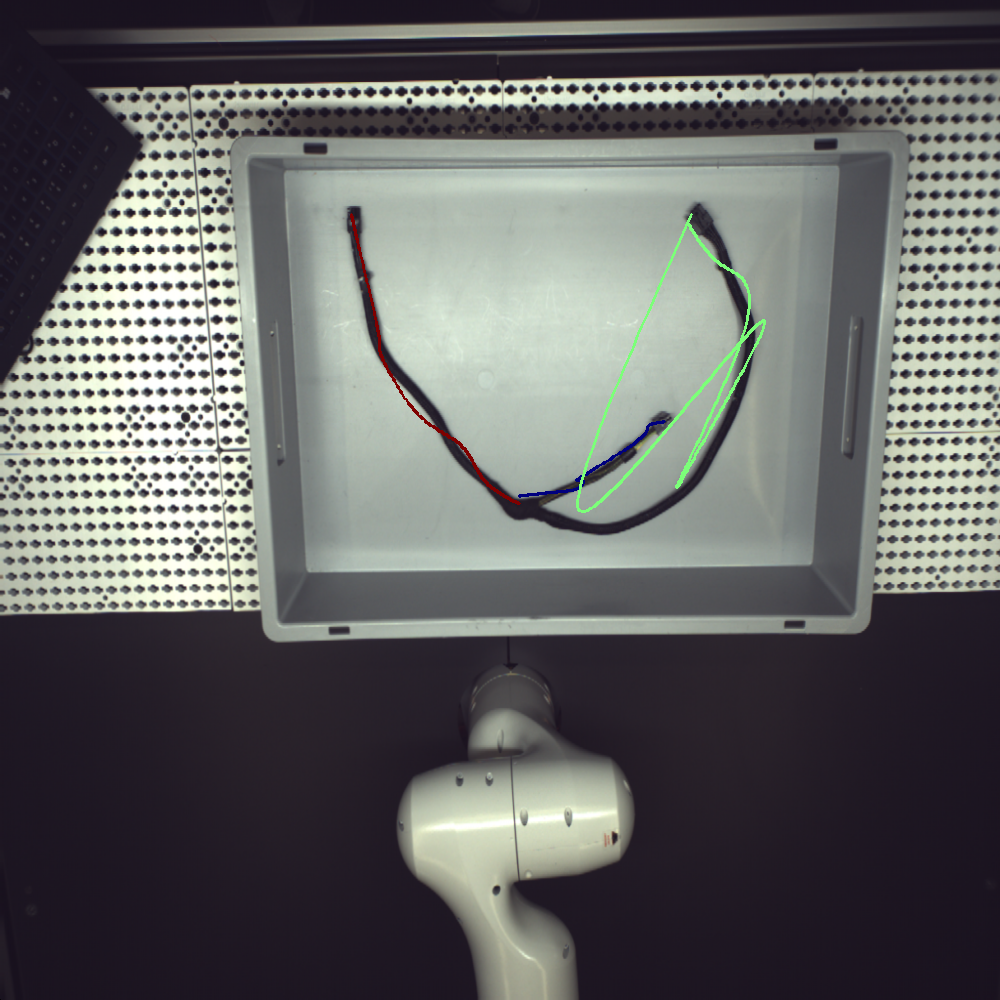
\includegraphics[width=0.6\linewidth]{example_images/keypoints_100_eval_withAttn}
	\caption{Validation for model with self attention}
	\label{fig:Training result validation Attention}
\end{figure}
The detection of keypoints is preciser than before. However, the sequence is still not correct.
To solve this problem, the keypoints are sorted before evaluation by using greedy algorithm. The keypoints are always gathered 
at the intersection at the beginning. Thus, the first point in the sequence of keypoints can be easily determined. After that the 
next point nearest to the first point will be found. Once this step has been done, the previous point is excluded from the list of 
following points to be searched. The point closest to the newly found point will continue to be found. This process is repeated 
until all the keypoints have been iterated. After the sort of keypoints, the result of evaluation is \autoref{fig:Training result validation Attention and Sort}.\\
\begin{figure}
	\centering
	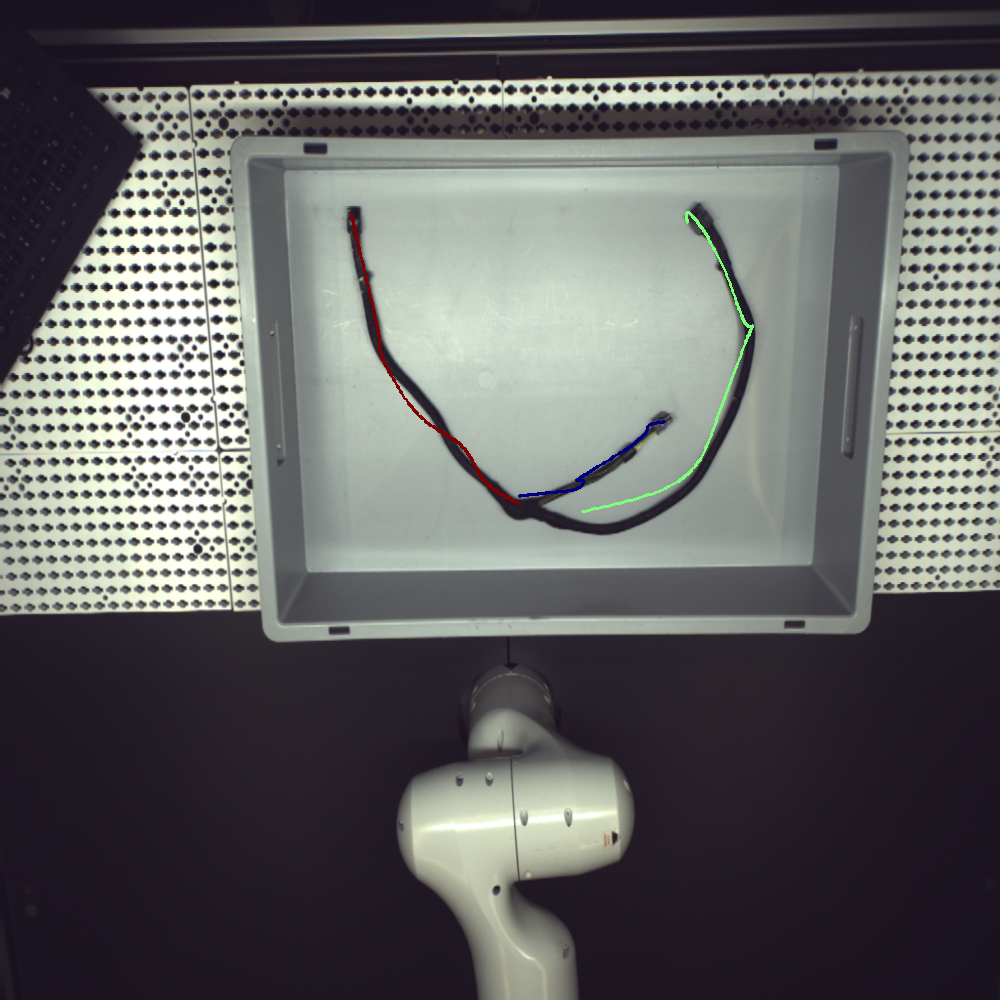
\includegraphics[width=0.6\linewidth]{example_images/withAttn_sort_keypoints_100_eval}
	\caption{Validation for model with sort of key points}
	\label{fig:Training result validation Attention and Sort}
\end{figure}
The keypoints are still at the same position, but the sequence of keypoints on each segment is sorted and the evaluation looks more reasonable. 
\subsection{Comparative experiment}
Several comparative experiments are done for evaluating the model.\\ 
\subsubsection{Resnet-50 as backbone}
Resnet-50 is used as the backbone to extract features in the first comparative experiment. The model is the nothing different but just the backbone is 
replaced. After the backbone, the dimension of the image changes from 1x3x256x256 to 1x2048x32x32. The validated loss will be decreased to 0.79 after 
177 epochs. The loss is $16\%$ higher than the model employed swin-transformer as backbone.  
\subsubsection{Resnet-50 as backbone}
Resnet-50 is used as the backbone to extract features in the first comparative experiment. The model is the nothing different but just the backbone is 
replaced. After the backbone, the dimension of the image changes from 1x3x256x256 to 1x2048x32x32. The validated loss will be decreased to 0.79 after 
177 epochs.
\subsubsection{YOLOV8}
YOLO V8 is a one stage object detection algorithm. The model after training could also predict the keypoints by using the coordinate regression method.
In contrast to the Heatmap method, the model predicts the coordinate of keypoints directly and compares it with the groundtruth. The dataset for YOLO is 
different from the dataset for the previous model. Each annotation file is in txt format and has one class "wire harness" and for each class there are eight 
keypoints, so after the training the model could also predict each segment individually. The model is still trained with the 100 images of wire harness.
The results are in \autoref{tab:Training results of YOLO}. The loss of validation is about 7 times higher than training loss and the model is over-fitting.
The generalization of the model is worse than the previous. \\
\begin{table}[htb]
    \centering
    \begin{tabular}{@{}llr@{}} \toprule
    \multicolumn{2}{c}{Result}             \\ \cmidrule(r){1-2}
                 & Loss   \\ \midrule
        Training & 0.9    \\
        Validation& 6.5    \\ \bottomrule
    \end{tabular}
    \caption{Training results of YOLO} 
    \label{tab:Training results of YOLO}
    \end{table}
In order to test the coordinate regression method further, inspired by YOLO, the head of the previous model was modified to use the coordinate regression method.
The Dataset is the same and after the training, the validation loss is double of the previous validation loss. At least for small dataset, the coordinate regression
method is not suitable.
\subsection{Dataset expansion}
Using a small dataset like previous is good for fast verifying the idea. However, a dataset that is too small may lead to: 
\begin{itemize}
	\item Overfitting
	\item High Variance of the model parameters
	\item Difficult in evaluation
	\item Inaccurate model predictions
\end{itemize}
Therefore, it is essential to find ways to expand the dataset. In this subsection, we experiment with two methods for expanding the dataset. They are:
1) Wire bundle images generated by CycleGAN. 2) Composition of new wire harness images by rotating, translating on the branches of the original image. 
The models are pre-trained using the two methods, respectively. After obtaining satisfactory results, the model is subjected to transfer learning using 
the previous dataset to explore whether the pre-training has improved the predictive ability of the model.
\subsubsection{Expand Dataset by CycleGAN}
Generating the virtual images of the wire harness using the CycleGAN network requires first generating images of the simple three-branched-spline curve 
obtained by sketching \autopageref{fig:Spline}. Then the images of spline will be feed into the network for unsupervised learning. The model will output the virtual images of 
wire harnesses, which have the same shape of spline but with texture of real wire harnesses\autoref{fig:fakeimage}.
\begin{figure}
	\centering
	
\includegraphics[width=0.6\linewidth]{example_images/CycleGAN_spline}
	\caption{Spline}
	\label{fig:Spline}
\end{figure}

\begin{figure}
	\centering
	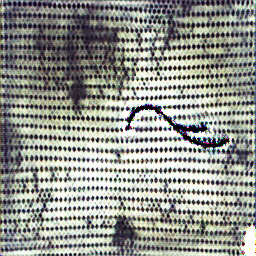
\includegraphics[width=0.6\linewidth]{example_images/CycleGAN_fakeimage}
	\caption{fakeimage}
	\label{fig:fakeimage}
\end{figure}
After training with the 2000 virtual images created by CycleGAN network, the prediction results are in \autoref{Pretraining Results}.
\begin{figure}
	\centering
	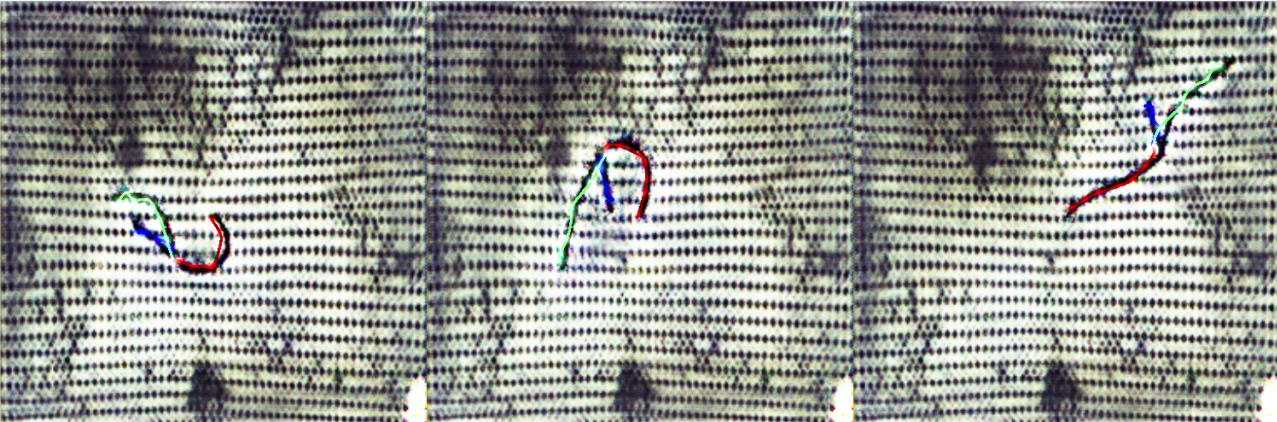
\includegraphics[width=0.6\linewidth]{example_images/PretrainingResultCycleGAN}
	\caption{Validation Results of pretraining}
	\label{Pretraining Results}
\end{figure}
And the model is trained again with the real images by transfer learning. The validation loss is $20\%$ lower than not using pretraining. An example of validated result is 
\autoref{Validation Results using transfer learning}
\begin{figure}
	\centering
	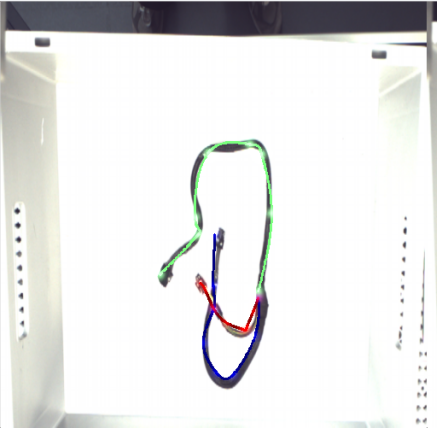
\includegraphics[width=0.6\linewidth]{example_images/usePretraining_NoTransformer}
	\caption{Validation Results of model using transfer learning}
	\label{Validation Results using transfer learning}
\end{figure}


\subsubsection{Expand Dataset by operations on segments} 
To operate on the branches of the harness, the harness first needs to be segmented. Here the images are firstly segmented to individual segments by using
Label-Studio, see \autoref{fig:Wire Segmentation}.\\
\begin{figure}
	\centering
	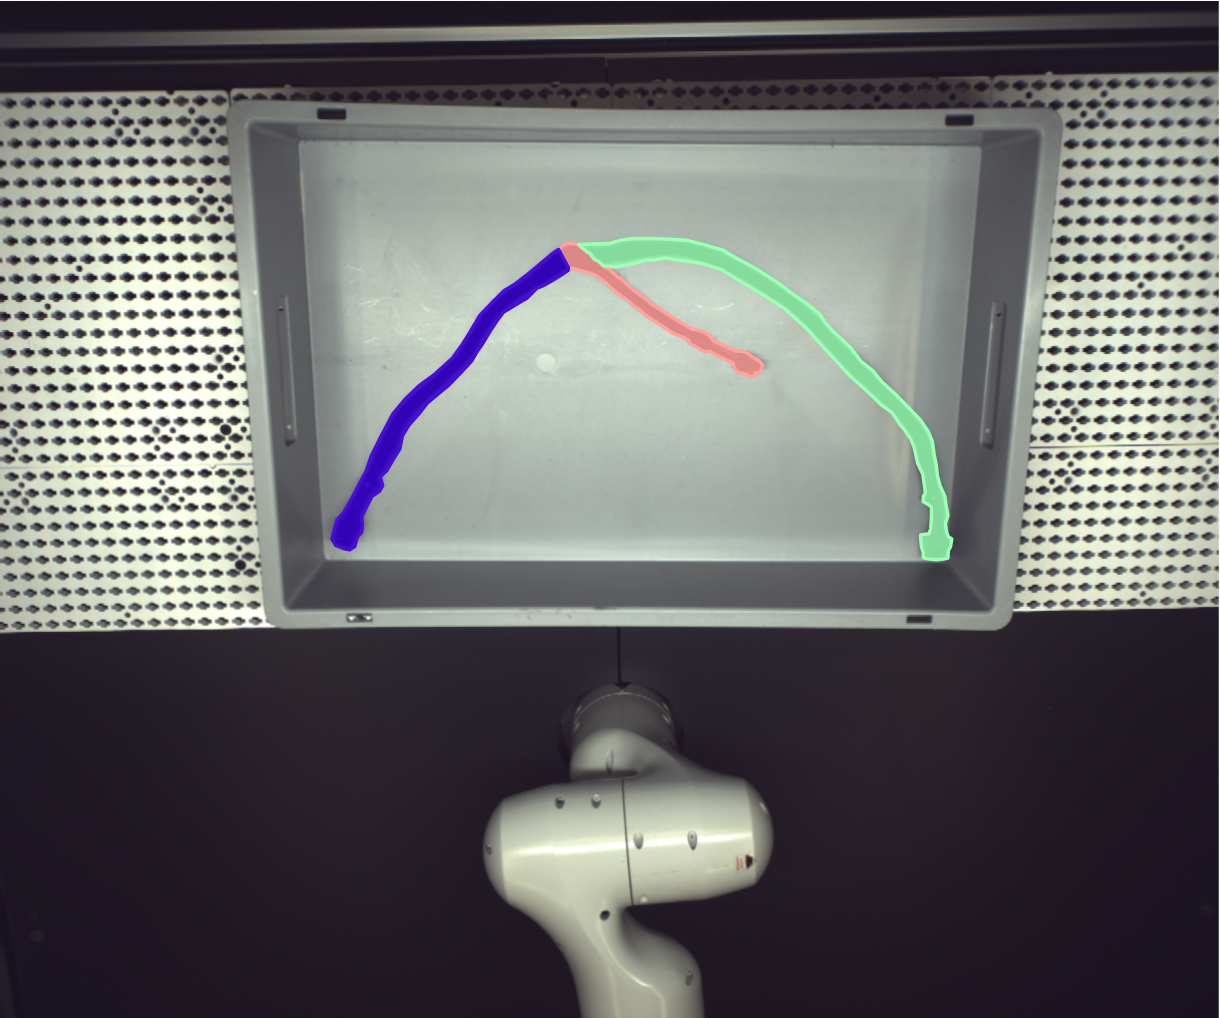
\includegraphics[width=0.6\linewidth]{example_images/img_0_segment}
	\caption{Wire Segmentation}
	\label{fig:Wire Segmentation}
\end{figure}
A rotation matrix is defined as \autoref{eq:rotation matrix}:
\begin{align}
	\begin{bmatrix}
		cos(\theta)&  -sin(\theta )&x \\
		sin(\theta )&  cos(\theta )&y  \\
		0&  0&1
	  \end{bmatrix} \label{eq:rotation matrix}
\end{align}
An all-zeros mask will be created firstly that has the same size as the image of wire harnesses. The values on mask, where corresponds to the coordinate position of
annotated points of segmentation, are then equal to one. The corresponding image region $\mho$ of the wire harness will be segmented as a polygonal region based on the mask.
Build the rotation matrix relative to the desired position and then calculate its corresponding new coordinates by using \autoref{eq:new region}. 
Paste the previously segmented polygonal area onto the empty background. The new generated virtual image is \autoref{fig:fake image}.
\begin{align}
	\mho ^{\star } = \mho \cdot \begin{bmatrix}
		cos(\theta)&  -sin(\theta )&x \\
		sin(\theta )&  cos(\theta )&y  \\
		0&  0&1
	  \end{bmatrix} \label{eq:new region}
\end{align}

\begin{figure}
	\centering
	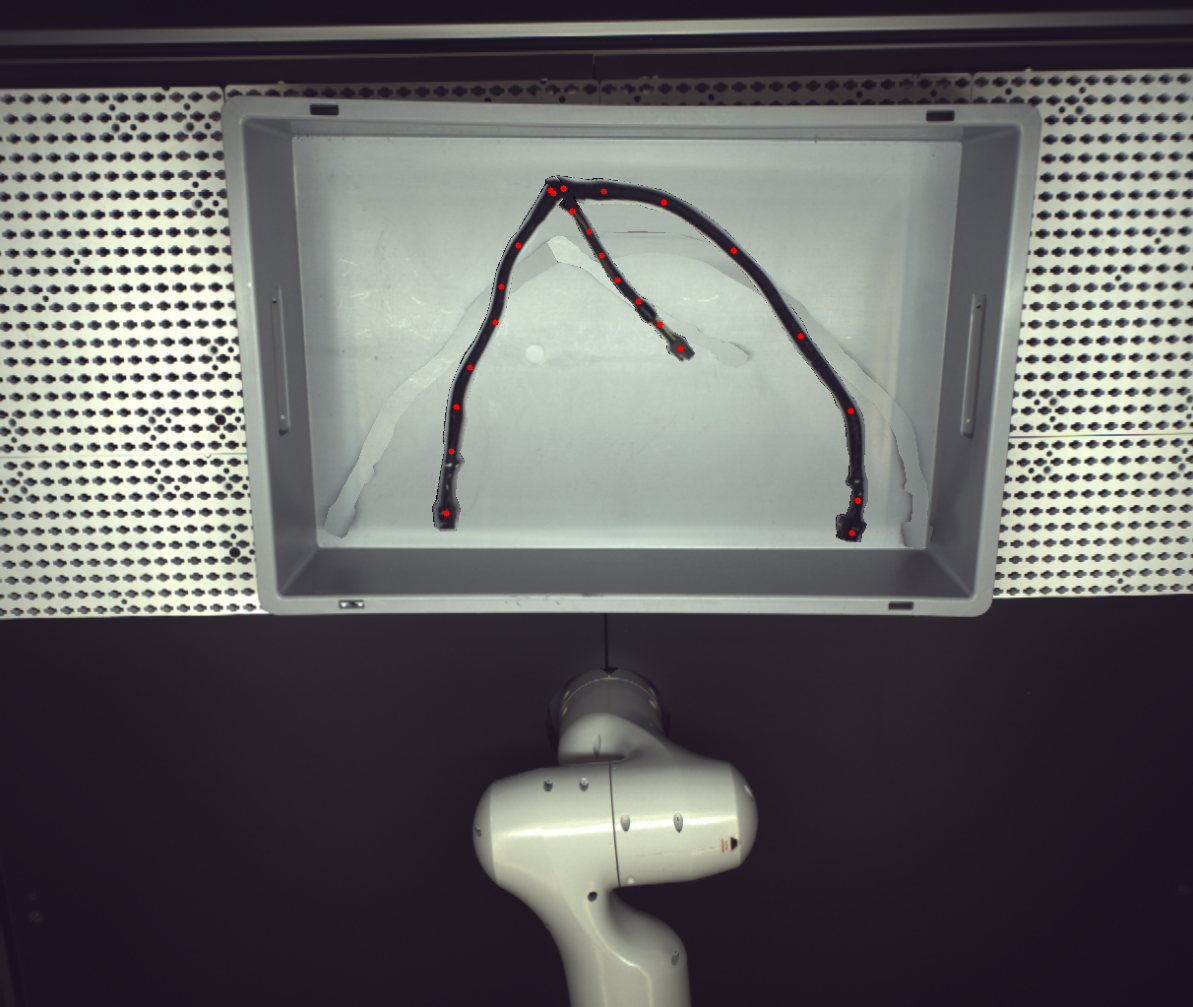
\includegraphics[width=0.6\linewidth]{example_images/img_0_segment_fakeImages}
	\caption{fake image}
	\label{fig:fake image}
\end{figure}
The corresponding annotation $\Theta $ could also be calculated with the rotation matrix as \autoref{eq:new anno}:
\begin{align}
	\Theta ^{\star } = \Theta \cdot \begin{bmatrix}
		cos(\theta)&  -sin(\theta )&x \\
		sin(\theta )&  cos(\theta )&y  \\
		0&  0&1
	  \end{bmatrix} \label{eq:new anno}
\end{align}

    
    
    \chapter{Conclusions}

    % ********************************************************************
    % End of contents
    % ********************************************************************
    
    \cleardoublepage
    \printbibliography
    
     \cleardoublepage
    \cleardoublepage
\chapter*{Abkürzungsverzeichnis}

\begin{acronym}[SPS] % longest acronym in [...] for spacing
    % \acro{short}{long}
    % \acroextra{...} wird nur im Abkürzungsverzeichnis ausgegeben.
    \acro{ISW}{Institut für Steuerungstechnik der Werkzeugmaschinen und Fertigungseinrichtungen \acroextra{der Universität Stuttgart}}
    \acro{SPS}{Speicherprogrammierbare Steuerung}
    % acrodefplural, wenn eine Pluralform benötigt wird (Standard: angehängtes "s" aus dem Englischen)
    % \acrodefplural{acroKey}[plural short]{plural long}
    \acrodefplural{SPS}[SPS]{Speicherprogrammierbare Steuerungen}

\end{acronym}
    
    \cleardoublepage
    \listoffigures
    
    \cleardoublepage
    \listoftables
    
    \cleardoublepage
\addchap{List of Symbols}

This section is optional. 
Ask your supervisor whether it is required for your thesis. 
If you have more than 10 formulas involved it probably is.

There are two ways to build a list of symbols:

\begin{itemize}
    \item If you just want to get it done, then use a \texttt{longtable} and fill your symbols in, see table below.
    \item If you want it fancy, then package \texttt{glossaries} (maybe \texttt{glossaries-extra}) may be your way to go. 
    Be warned that although it automates symbol handling (e.g. sorting and referencing of symbols), it comes with some administrative overhead. 
    You can find a discussion on different ways to achieve this \href{https://tex.stackexchange.com/a/366282}{on https://tex.stackexchange.com/a/366282}.
\end{itemize}
\centering
\begin{longtable}{@{}c l p{10cm}@{}}
\toprule
Symbol & Unit & Description \\
\midrule
\endfirsthead
\multicolumn{3}{c}{\textit{List of Symbols -- continued}}\\
\toprule
Symbol & Unit & Description \\
\midrule
\endhead
\bottomrule \multicolumn{3}{r}{\textit{Continued on next page}} \\
\endfoot
\bottomrule
\endlastfoot

% start here with your symbols:
\(\psi\) & rad & Heading angle of hamster \\
\(\dot x\) & m/s & Linear velocity of hamster \\
\(\ddot x_0\) & m/s$^2$ & Initial acceleration of hamster \\
\end{longtable}
    
    % Appendix, if needed:
    \appendix
    \chapter{Example appendix chapter}


\end{document}